\documentclass[
	% -- opções da classe memoir --
	12pt,				% tamanho da fonte
	openright,			% capítulos começam em pág ímpar (insere página vazia caso preciso)
	oneside,			% para impressão em recto e verso. Oposto a oneside
	a4paper,			% tamanho do papel.
	sumario=tradicional, % indenta o sumario 
	% -- opções da classe abntex2 --
	%chapter=TITLE,		% títulos de capítulos convertidos em letras maiúsculas
	%section=TITLE,		% títulos de seções convertidos em letras maiúsculas
	%subsection=TITLE,	% títulos de subseções convertidos em letras maiúsculas
	%subsubsection=TITLE,% títulos de subsubseções convertidos em letras maiúsculas
	% -- opções do pacote babel --
	english,			% idioma adicional para hifenização
	brazil,				% o último idioma é o principal do documento
	]{abntex2}

% ---
% PACOTES
% ---

% ---
% Pacotes fundamentais 
% ---
%\usepackage{lmodern}           % Usa a fonte Latin Modern
\usepackage{pslatex}            % Usa a fonte Times New Roman 
\usepackage[T1]{fontenc}		% Selecao de codigos de fonte.
\usepackage[utf8]{inputenc}		% Codificacao do documento (conversão automática dos acentos)
\usepackage{indentfirst}		% Indenta o primeiro parágrafo de cada seção.
\usepackage{color}				% Controle das cores
\usepackage{graphicx, draftfigure}			% Inclusão de gráficos
\usepackage{microtype} 			% para melhorias de justificação
\usepackage{amsfonts}			% para símbolos matemáticos
\newtheorem{theorem}{Teorema}[section]
\newtheorem{corollary}{Corollary}[theorem]
\newtheorem{lemma}[theorem]{Lemma}
\newtheorem{definition}{Definição}
\usepackage{algorithm}
\usepackage{algorithmic}
\usepackage{subfig}
\usepackage{hyperref}
\usepackage{lscape}
\usepackage{amsmath}
\usepackage{amssymb}
\usepackage{lscape}
\usepackage{caption}
\usepackage{listings}
\usepackage{xcolor}
\usepackage{xspace}
\usepackage{placeins}
%\usepackage[titletoc]{appendix}
% --- centralizador de tabelas -----
\newcolumntype{P}[1]{>{\centering\arraybackslash}p{#1}}
% ---
% Pacotes adicionais, usados apenas no âmbito do Modelo Canônico do abnteX2
% ---
\usepackage{lipsum}				% para geração de dummy text
% ---

% ---
% Pacotes de citações
% ---
\usepackage[brazilian,hyperpageref]{backref}	 % Paginas com as citações na bibl
\usepackage[alf]{abntex2cite}	% Citações padrão ABNT

% --- 
% CONFIGURAÇÕES DE PACOTES
% --- 

% ---
% Configurações do pacote backref
% Usado sem a opção hyperpageref de backref
\renewcommand{\backrefpagesname}{Citado na(s) página(s):~}
% Texto padrão antes do número das páginas
\renewcommand{\backref}{}
% Define os textos da citação
\renewcommand*{\backrefalt}[4]{
	\ifcase #1 %
		Nenhuma citação no texto.%
	\or
		Citado na página #2.%
	\else
		Citado #1 vezes nas páginas #2.%
	\fi}%
% ---

% ---
% Informações de dados para CAPA e FOLHA DE ROSTO
% ---
\titulo{Análise qualitativa do modelo de gravidade global EIGEN-6C4 na modelagem de distúrbios de gravidade sob a região da Bacia do Parnaíba}
\orientador{Dr. Kristoffer A.T.Hallam}
\coorientador{Dr. Rodrigo Bijani}
\autor{Allan Soares Ramalho}
\local{Brasil}
\data{\today}
\instituicao{Universidade Federal Fluminense - UFF
  \par
  Departamento de Geologia e Geofísica
  \par
  Graduação em Geofísica}
\tipotrabalho{Projeto de pesquisa}
% O preambulo deve conter o tipo do trabalho, o objetivo, 
% o nome da instituição e a área de concentração 
\preambulo{Projeto Final de Graduação apresentado ao curso de graduação em Geofísica da Universidade Federal  Fluminense  como  requisito  para  a obtenção  do  grau  de  Bacharel  em  Geofísica.}
% ---
% ---
% Configurações de aparência do PDF final

% alterando o aspecto da cor azul
\definecolor{blue}{RGB}{41,5,195}

% informações do PDF
\makeatletter
\hypersetup{
     	%pagebackref=true,
		pdftitle={\@title}, 
		pdfauthor={\@author},
    	pdfsubject={\imprimirpreambulo},
	    pdfcreator={LaTeX with abnTeX2},
		pdfkeywords={abnt}{latex}{abntex}{abntex2}{projeto de pesquisa}, 
		colorlinks=true,       		% false: boxed links; true: colored links
    	linkcolor=black,          	% color of internal links
    	citecolor=black,        		% color of links to bibliography
    	filecolor=magenta,      		% color of file links
		urlcolor=blue,
		bookmarksdepth=4
}
\makeatother

% --- 

% --- 
% Espaçamentos entre linhas e parágrafos 
% --- 

% O tamanho do parágrafo é dado por:
\setlength{\parindent}{1.3cm}

% Controle do espaçamento entre um parágrafo e outro:
\setlength{\parskip}{0.2cm}  % tente também \onelineskip

% ---
% compila o indice
% ---
\makeindex
% ---

% ----
% Início do documento
% ----
\begin{document}

\begin{flushleft}
	\vspace*{-0.7mm}
	\setlength\baselineskip{-10mm}
	\setlength\parskip{-10.mm}
	\makebox[20mm][c]{\hspace{13.5cm}\includegraphics[width=3cm]{figs/brasaouff}}
\end{flushleft}
\vspace{\fill}

% Seleciona o idioma do documento (conforme pacotes do babel)
%\selectlanguage{english}
\selectlanguage{brazil}
% Retira espaço extra obsoleto entre as frases.
\frenchspacing



% ----------------------------------------------------------
% ELEMENTOS PRÉ-TEXTUAIS
% ----------------------------------------------------------
% \pretextual

% ---
% Capa
% ---
\imprimircapa
% ---

% ---
% Folha de rosto
% ---
\imprimirfolhaderosto
% ---

% folha de aprovação:
\begin{folhadeaprovacao}
  \begin{center}
    {\ABNTEXchapterfont\Large\imprimirautor}
    \vspace*{\fill}\vspace*{\fill}
    \begin{center}
      \ABNTEXchapterfont\bfseries\Large\imprimirtitulo
    \end{center}
    \vspace*{\fill}
    
    \hspace{.45\textwidth}
    \begin{minipage}{.50\textwidth}
        \imprimirpreambulo
    \end{minipage}%
   \vspace*{\fill}
   \end{center}
        
   Comitê composto pelos seguintes avaliadores:

   \assinatura{\textbf{\imprimirorientador} (Orientador) \\  ON - MCTIC}
   \assinatura{\textbf{\imprimircoorientador} (Coorientador) \\ GIECAR/GGO - UFF} 
   \assinatura{\textbf{Dr. André Luis Albuquerque dos Reis} \\  ON - MCTIC}
   \assinatura{\textbf{MSc. Larissa da Silva Piauilino} \\  ON - MCTIC}
   
   \begin{center}
       \vspace*{0.5cm}
       {\large\imprimirlocal}
       \par
       {\large\imprimirdata}
       \vspace*{1cm}
   \end{center} 
\end{folhadeaprovacao}
% ---
% NOTA DA ABNT NBR 15287:2011, p. 4:
%  ``Se exigido pela entidade, apresentar os dados curriculares do autor em
%     folha ou página distinta após a folha de rosto.''
% ---

% ---
% inserir lista de ilustrações
% ---
\pdfbookmark[0]{\listfigurename}{lof}
%\listoffigures*
\cleardoublepage
% ---

% ---
% inserir lista de tabelas
% ---
\pdfbookmark[0]{\listtablename}{lot}
%\listoftables*
\cleardoublepage
% ---
\begin{agradecimentos}
A Deus, por me trazer até este momento e me dar forças ao longo de toda trajetória.

À minha esposa, Adriana, que sempre esteve ao meu lado em todos os momentos. Foi companheira, amiga, conselheira, mas principalmente me apoiou e incentivou nos momentos mais difíceis que eu pensei em desistir. Esse momento também é seu, se cheguei aqui foi por ter você ao meu lado.

À minha mãe, Rita, por todo empenho e dedicação. Com toda certeza a educação e o caráter tenho é reflexo da mulher guerreira e forte que você sempre foi. Nunca vou me esquecer todo o sacrifício e de tudo que você abriu mão, espero um dia conseguir retribuir toda essa dedicação e amor.

Ao meu pai, Márcio, por todo o suporte que deu a minha educação e pelas orientações. Agradeço a Deus por tudo que você é na minha vida e pela oportunidade que Ele nos deu. 

Aos meus irmãos que sempre me apoiaram.

Aos meus orientadores, Kristoffer e Bijani, por aceitarem a difícil tarefa de me orientar, não facilitei a vida de vocês. Agradeço por toda a paciência, dedicação, ajuda e compreensão. Vocês foram fora de série, se dispuseram em me ajudar em todos os momentos e sempre me incentivaram. Admiro muito os dois, vocês se tornaram espelho para minha vida profissional e acadêmica.

Aos meus professores da graduação, por toda dedicação empreendida ao longo destes anos.

À Universidade Federal Fluminense, por prover professores extremamente competentes e humanos. 

Aos amigos que adquiri ao longo desses anos de faculdade, dentre eles em especial ao Ammir Karsou e Diogo Ceddia, por me apoiarem com dicas e dúvidas em relação a programação. Vocês contribuíram muito e sou bastante grato.
\end{agradecimentos}
% ---
\begin{epigrafe}
	\vspace*{\fill}
	\begin{flushright}
		\textit{“Quem dá os primeiros passos na análise de observações começa por fazer uma concessão: abdicar da pretensão de obter o verdadeiro valor de uma grandeza medida.” \newline
			Camil Gemael}
	\end{flushright}
\end{epigrafe}         
% ---
% inserir lista de abreviaturas e siglas
% ---
%\begin{siglas}
%\item[ABNT] Associação Brasileira de Normas Técnicas
%\item[abnTeX] ABsurdas Normas para TeX
%\end{siglas}
% ---

% ---
% inserir lista de símbolos
% ---
%\begin{simbolos}
%\item[$ \Gamma $] Letra grega Gama
%\item[$ \Lambda $] Lambda
%\item[$ \zeta $] Letra grega minúscula zeta
%\item[$ \in $] Pertence
%\end{simbolos}
% ---
% Keywords command
\providecommand{\keywords}[1]
{
	\small	
	\textbf{\textit{Palavras chave: }} #1
}
\begin{center}
{\Huge Resumo}
\end{center}	
Neste trabalho, foi realizado um estudo comparativo entre dois conjuntos de dados de distúrbio de gravidade sobre a região da Bacia do Parnaíba: o primeiro refere-se aos distúrbios terrestres adquiridos pelo Observatório Nacional; o segundo é proveniente do modelo de gravidade global \textit{EIGEN-6C4}, onde um compilado de dados de gravidade terrestres, aéreos, marinhos e de satélite são utilizados no cálculo dos coeficientes da expansão em harmônicos esféricos. Os levantamentos gravimétricos são extremamente importantes para a geofísica aplicada, por fornecerem meios de avaliar e inferir informações relevantes sobre a distribuição de densidade interna da Terra. Esses levantamentos diferem na forma de aquisição, seja terrestre ou transportada, e na cobertura de dados. A depender do acesso à regiões remotas, a gravimetria terrestre pode ser proibitiva, o que acarreta em uma limitação na cobertura espacial dos dados. Como alternativa para essa limitação surge a gravimetria transportada. No entanto, os dados obtidos nesse tipo de aquisição podem apresentar ruídos indesejáveis por consequência das oscilações e vibrações dos veículos empregados. A utilização de um modelo global supre tais limitações, uma vez que esses modelos permitem calcular valores de gravidade em qualquer ponto do globo. Dessa forma, é possível descrever o campo de gravidade em qualquer ponto da Terra. Apesar disso, sua aplicação requer uma análise mais cuidadosa, devido às limitações associadas ao trucamento da série harmônica e às grandes distâncias entre os satélites e a subsuperfície investigada. Neste trabalho foi apresentada uma análise qualitativa baseada na comparação entre gravimetria terrestre e  de satélite. Para tal, foi calculado o vetor de resíduos entre os distúrbios de gravidade terrestres e os calculados via modelo, chamados aqui de observados e preditos, respectivamente. Os histogramas dos resíduos apresentaram média positiva e desvio padrão relativamente elevados, o que indica uma subestimativa dos distúrbios de gravidade. Isso pode estar relacionado à baixa amostragem dos dados utilizados neste trabalho. Outro potencial motivo consiste da não inclusão de dados terrestres e aéreos ao modelo na região estudada, o que acarreta em um aumento das feições irrealistas nos distúrbios preditos. Um terceiro fator bastante relevante é o truncamento da série harmônica, que pode ser decisivo para justificar os resíduos apresentados neste estudo.


\noindent{\keywords{gravimetria; distúrbio de gravidade; modelo de gravidade global.}}






% Keywords command
\providecommand{\keywordss}[1]
{
	\small	
	\textbf{\textit{Keywords: }} #1
}
\begin{center}
	{\Huge Abstract}
\end{center}
In this work, a comparative study was carried out between two sets of gravity disturbance data on the Parnaíba Basin region: the first refers to terrestrial disturbances acquired by the National Observatory; the second comes from the global gravity model \textit{EIGEN-6C4}, where a compilation of terrestrial, aerial, marine and satellite gravity data is used to calculate the expansion coefficients in spherical harmonics. Gravimetric surveys are extremely important for applied geophysics, as they provide a means of evaluating and inferring relevant information about the Earth's internal density distribution. These surveys differ in the form of acquisition, whether overland or transported, and in data coverage. Depending on access to remote regions, terrestrial gravimetry can be prohibitive, which results in a limitation in the spatial coverage of the data. As an alternative to this limitation, transported gravimetry appears. However, the data obtained in this type of acquisition can present undesirable noises due to the oscillations and vibrations of the vehicles used. The use of a global model overcomes these limitations, since these models allow the calculation of gravity values anywhere in the globe. In this way, it is possible to describe the gravity field at any point on Earth. Despite this, its application requires a more careful analysis, due to the limitations associated with the harmonic series truncation and the great distances between the satellites and the investigated subsurface. In this work, a qualitative analysis based on the comparison between terrestrial and satellite gravimetry was presented. For this purpose, the vector of residuals was calculated between terrestrial gravity disturbances and those calculated via the model, called here observed and predicted, respectively. The residual histograms showed a relatively high positive mean and standard deviation, which indicates an underestimation of the gravity disturbances. This may be related to the low sampling of data used in this work. Another potential reason is that land and air data are not included in the model in the studied region, which leads to an increase in unrealistic features in the predicted disturbances. A third very relevant factor is the truncation of the harmonic series, which can be decisive to justify the residues presented in this study.

\noindent{\keywordss{gravimetry; gravity disturbance; global gravity model.}}	






% ---
% inserir o sumario
% ---
\pdfbookmark[0]{\contentsname}{toc}
\tableofcontents*
\cleardoublepage

% ---
\textual

% ----- Inicio do documento -----------:
% -------------- Lista de figuras: --------------------------------
\listoffigures	
\listoftables

% Capitulos:

% ------------------- capitulo 1:
\chapter{Introdução}

A gravimetria é um método geofísico que tem por objetivo determinar a aceleração da gravidade da Terra sobre ou próximo à sua superfície \cite{torge1989}. Dentro desse escopo, os levantamentos gravimétricos contribuem significativamente para estudos geológicos e geofísicos, pois geram meios de avaliar e inferir sobre a distribuição de densidade interna da Terra. O Observatório Nacional (ON) é a instituição brasileira pioneira em gravimetria e, em 1978, passou a ser responsável pela implantação e manutenção da Rede Gravimétrica Fundamental Brasileira (RGFB). Dessa forma, desde o fim da década de 70, o ON opera e mantém em todo o país a RGFB, disponibilizando um conjunto de estações gravimétricas terrestres de alta precisão que servem de apoio para os levantamentos gravimétricos conduzidos no Brasil \cite{escobar1987rede,subiza2001,castro2018}. A partir da segunda metade do século XX, começou a ser implementada a gravimetria transportada, aérea e náutica, que possibilitavam adquirir os dados em lugares remotos e de acesso mais restrito à gravimetria terrestre \cite{halpenny1995airborne,bell1999airborne}. De acordo com \citeonline{carbonari2007}, as aquisições aéreas e marinhas tem a vantagem de adquirir um maior conjunto de dados com uma velocidade consideravelmente maior do que no caso terrestre, podendo cobrir uma vasta área de investigação. No entanto, as oscilações verticais e horizontais causadas pela movimentação dos veículos podem gerar ruídos indesejáveis nas medidas. 

Em 1976, foi lançado o primeiro satélite de estudo geodinâmico com o objetivo de determinar o formato da Terra, iniciando a era dos satélites gravitacionais. Esse satélite, denominado LAGEOS (\textit{Laser Geodynamics Satellite}), consiste em uma esfera metálica de $60$ centímetros de diâmetro com $426$ refletores a laser e nenhum instrumento a bordo. Foi posicionado em uma órbita de $5900$ quilômetros de altitude e fornece medições da reflexão dos feixes de luz emitidos da Terra ao longo do tempo. Posteriormente, em 2000, foi lançada a missão CHAMP (\textit{Challenging Minisatellite Payload}), a primeira das modernas missões de satélites que possibilitou um detalhamento sem precedentes do campo gravitacional e magnético terrestre \cite{lobianco2005}, através de instrumentos embarcados como acelerômetro, magnetômetro, sensor inercial, retrorrefletor de raios laser e receptor  $GNSS$ (\textit{Global Navigation Satellite System}). De acordo com o mesmo autor, o satélite esteve em órbita a uma altitude inicial de $454$ quilômetros, e, visando realizar estudos mais densos sobre o campo de gravidade, teve sua altitude alterada para $300$ quilômetros. Foi a primeira vez que um satélite com receptores GNSS orbitou a baixas altitudes, permitindo que o seu posicionamento ocorresse com a precisão de poucos centímetros \cite{schwintzer2002}. Em 2002, foi lançada a missão GRACE (\textit{Gravity Recovery and Climate Experiment}), composta por dois satélites gêmeos do tipo CHAMP, desenvolvida para o estudo das variações temporais do campo gravitacional da Terra \cite{torge2001geodesy,schwintzer2002}. Sua órbita inicial era de aproximadamente $500$ quilômetros. Mais tarde, em 2009, foi lançada a missão GOCE (\textit{Gravity Field and Steady-State Ocean Circulation Explorer}), a terceira das modernas missões satelitais, que teve como objetivo determinar o geoide com precisão de $\approx 2$ centímetros \cite{torge2001geodesy} e distúrbio de gravidade $\approx 2$ mGal \cite{junior2019evoluccao}. O projeto previa que o satélite estivesse em órbita com a menor altitude possível, a uma altura inicial aproximada de $260$ quilômetros e, posteriormente, de $235$ quilômetros. O principal instrumento da missão GOCE era o gradiômetro, que consistia num conjunto de acelerômetros de três eixos, que chegava a ser $100$ vezes mais sensível que os demais utilizados até então. 

As aquisições gravimétricas terrestres, apesar da resolução bastante acurada, apresentam dificuldades para serem realizadas em regiões de difícil acesso e em alguns casos podem ser inviáveis. Já as aquisições marinhas e aerotransportadas contornam esse tipo de problema. No entanto, possuem custo relativamente alto e apresentam o problema de serem utilizadas sobre plataformas móveis que influenciam diretamente nos dados \cite{carbonari2007, castro2018}. As aquisições de satélites apresentam cobertura global, amostragem relativamente alta, são regularmente espaçadas e sua utilização permite calcular a gravidade em qualquer ponto do globo. Os dados de gravidade adquiridos, através das diferentes formas possíveis, contribuem para a interpretação geofísica. Segundo \citeonline{hackney2003}, a diferença da gravidade real da Terra e a gravidade teórica resulta em anomalias e distúrbios de gravidade, sendo os conceitos de distúrbio mais difundidos sob a perspectiva geodésica e os conceitos de anomalia sob a perspectiva geofísica. Por exemplo, \citeonline{carbonari2007} mostra a utilização de anomalias de gravidade para conhecimento geológico da bacia Sergipe-Alagoas e sua aplicabilidade, na exploração de hidrocarbonetos, a fim de delimitar as principais feições estruturais, ajudando a compreender a evolução da bacia. Já \citeonline{disturbios_investig} utilizou distúrbios de gravidade para auxiliar no processo de investigação geofísica da interface entre crostas oceânica e continental na Elevação do Ceará. Para isso, é utilizada a teoria da inversão e a modelagem usando prismas justapostos. \citeonline{uieda2017} utilizou os distúrbios de gravidade na estimativa da descontinuidade de Mohorovičić (Moho) na região da América do Sul. \citeonline{marcela} utilizou distúrbios de gravidade para estimar simultaneamente as geometrias do embasamento e do Moho, bem como a profundidade do Moho de referência ao longo de um perfil que cruza uma margem passiva estriada da Bacia de Pelotas.

% Falar como se obtem os modelos de gravidade(nada extenso, colocar uma referencia)
Uma das mais relevantes atribuições de um geofísico é ser capaz de reproduzir um conjunto de dados. Dessa forma, muitas respostas podem ser obtidas de forma rápida e eficiente. Logo, a modelagem gravimétrica apresenta-se como uma poderosa ferramenta de trabalho. Em escala global, é comum a utilização dos harmônicos esféricos e funções \textit{spline} \cite{sandwell1987biharmonic}. Modelos de gravidade global (MGGs) descrevem de forma aproximada o campo de gravidade da Terra em um espaço tridimensional, através de expansões em harmônicos esféricos \cite{barthelmes2009}. De acordo com \citeonline{barthelmes2014global}, a aplicação de dados de satélites artificiais nos MGGs permitiu um significativo aprimoramento destes modelos. Os dados de satélites adquiridos principalmente através das missões LAGEOS, CHAMP, GRACE e GOCE contribuíram para o desenvolvimento de vários MGGs, marcando o início do século XXI como a década dos potenciais de gravidade \cite{barthelmes2014global,junior2019evoluccao}. Cada uma destas missões teve sua contribuição específica em termos de coeficientes de um MGG. Os dados do LAGEOS contribuíram para os baixos graus dos modelos, em torno de 5 \cite{torge2001geodesy}. De acordo com o mesmo autor, os dados da missão GRACE seriam utilizados para modelar a Terra no que diz respeito aos médios graus, até 150. Já as informações do GOCE modelam o planeta para os graus mais altos, em torno de 300 \cite{torge2001geodesy,forste2016}. Segundo \citeonline{reigber2003champ}, os dados obtidos na missão CHAMP deram origem a um MGG quatro vezes mais preciso que os anteriores, o \textit{EIGEN-2}, que foi desenvolvido em termos de harmônicos esféricos até grau e ordem $120$. Segundo \citeonline{junior2019evoluccao}, o primeiro MGG  com dados obtidos na missão GRACE apresentou resultados de 10 a 50 vezes mais precisos do que qualquer outro  MGG que atuasse em faixas de médios e/ou longos de comprimentos de onda. Os MGGs mais antigos expandem a série em harmônicos a grau e ordem  relativamente baixos, reflexo do desenvolvimento tecnológico e computacional de suas respectivas épocas. Já os modelos mais recentes, como o \textit{EGM2008} e o \textit{EIGEN-6C4} , apresentam valores relativamente altos de grau e ordem. Esse nível de detalhamento é atingindo por serem modelos combinados, isto é, além dos recursos computacionais e tecnológicos mais modernos, eles utilizam dados de satélites combinados com dados terrestres, aerotransportados e marinhos \cite{eigen,barbosagravimetria}.

Tendo em vista a temática abordada, o objetivo deste trabalho consiste na análise comparativa entre distúrbios de gravidade terrestre observados e preditos para a região da Bacia do Parnaíba. O conjunto de dados utilizados para elaboração dessa pesquisa são dados de altitude e de gravidade terrestres, que foram adquiridos e disponibilizados pelo ON, e dados modelados através do MGG \textit{EIGEN-6C4}. Para fins comparativos, utilizamos os mesmos pontos de observação para estimar altitudes e gravidades absolutas através do modelo disponível no ICGEM (International Centre for Global Earth Models). As altitudes geométricas foram utilizadas para calcular a gravidade normal, através da fórmula analítica da gravidade de \citeonline{li2001}. Posteriormente, calculam-se os distúrbios de gravidade pela diferença entre as gravidades absoluta e normal sob cada coordenada do levantamento terrestre. Visando complementar o estudo, os distúrbios preditos e observados foram comparados através de uma análise estatística, por meio de histogramas dos resíduos e gráficos de dispersão, tanto das altitudes geométricas quanto dos distúrbios de gravidade. 


% ------------------- capitulo 2:
\chapter{Fundamentação teórica}
\section{Sistemas de Referência}

Definir posições de um objeto ou alvo de estudo sobre a superfície terrestre requer um tratamento matemático \cite{d1999coordenadas}, a fim de estabelecer a localização em relação a uma origem. Os sistemas de coordenadas são definidos em termos da orientação, métrica e curvatura \cite{torge2001geodesy}. Dentre os sistemas de referência abordados na literatura, cuja nomenclatura pode ser distinta daquela apresentada neste estudo, destacam-se três que são os mais utilizados em geofísica aplicada. Todos eles seguem o movimento de rotação da Terra e são utilizados na descrição matemática das posições de objetos localizados sobre ou próximos à superfície terrestre \cite{torge}.

O \textit{Sistema Cartesiano Geocêntrico} $(SCG)$ faz uso do sistema de coordenadas ortogonais $\mathbf{XYZ}$, cuja origem coincide com o centro de massa da Terra. O eixo $\mathbf{Z}$ coincide com o eixo de rotação médio da Terra e, portanto, aponta para o polo norte, $\mathbf{X}$ aponta na direção  do meridiano médio de \textit{Greenwich} e $\mathbf{Y}$ é o eixo complementar segundo a regra da mão direita \cite{soler1976differential,soler1988,torge}, como exemplificado na Figura~\ref{fig:datum}.a.

O \textit{Sistema Geodésico Geocêntrico} (SGG) é largamente utilizado em sistemas de navegação por GPS (\textit{Global Positioning System}, \cite{cai2011}) e é definido de acordo com um modelo de elipsoide de referência usado para representar a Terra Normal. Este elipsoide é estabelecido uma vez que são fixados, principalmente, os semieixos maior e menor, $a$ e $b$, respectivamente, conservando, assim, o achatamento terrestre $(f)$ nos polos. Nesse sistema, a origem está localizada no centro do elipsoide de referência \cite{soler1976differential} e um ponto fictício $P$ na superfície terrestre é posicionado a partir de três coordenadas: altitude geométrica ($h$), que corresponde à distância do ponto $P$ à superfície  do elipsoide, medido na direção normal àquele; a latitude geodésica ($\varphi$), que é definida como o ângulo que a \textit{normal} ao elipsoide  forma com sua projeção equatorial; a longitude ($\lambda$), que é o ângulo diedro formado pelo meridiano de Greenwich e o meridiano passante pelo ponto $P$ como pode ser visto nas Figuras~\ref{fig:datum}.a e ~\ref{fig:datum}.b. Para cada ponto $(h,\varphi,\lambda)$, existem três vetores unitários ortogonais entre si, formando os eixos do sistema de coordenadas, definidos por \citeonline{soler1976differential}:

\begin{equation}
\label{eq:vetores_unitarios}
\displaystyle \mathbf{\hat{u}} = 
\left(\begin{array}{c}
\cos{\varphi} \cos{\lambda} \\ \cos{\lambda} \sin{\lambda}\\  \sin{\varphi}
\end{array} \right)  \quad ; \quad
\mathbf{\hat{v}} =
\left(\begin{array}{c}
-\sin{\varphi} \cos{\lambda} \\ -\sin{\varphi} \sin{\lambda} \\ \cos{\varphi}
\end{array} \right)  \quad ; \quad
\mathbf{\hat{w}} =
\left(\begin{array}{c}
-\sin{\lambda} \\ \cos{\lambda} \\ 0
\end{array} \right)
\end{equation} 

\begin{figure}[h]
	\centering
	\includegraphics[width=10cm,height=10cm]{figs/sistemas_de_referencia.png}
	\caption{ (a) e (b) são Sistema Cartesiano Geocêntrico ($SCG$) e Sistema Geodésico Geocêntrico ($SGG$), respectivamente. A posição de um ponto no $SCG$ é definida pelas coordenadas cartesianas geocêntricas ($X,Y,Z$), em que o eixo $Z$ coincide com o eixo médio de rotação da Terra, o eixo $X$ aponta para o Meridiano de Greenwich e o eixo $Y$ aponta para leste. O $SGG$ é definido por um esferoide oblato com semieixo maior $a$ e semieixo menor $b$. Neste sistema, a posição de um ponto é determinada pelas coordenadas geodésicas: altitude geométrica ($h$), latitude geodésica ($\varphi$) e longitude ($\lambda$). Os vetores unitários \textbf{û}, $\mathbf{\hat{v}}$ e \textbf{ŵ} definem direções ortogonais, em um determinado ponto. As quantidades associadas ao ponto $P$ estão indicadas com o subscrito $P$. Em (b), $Q$ representa um ponto sobre o elipsoide de referência na mesma latitude e longitude do ponto $P$. (c) é o Sistema Cartesiano Topocêntrico ($SCT$) com origem em um ponto $P$. Nesse sistema, a posição de um ponto é definida por coordenadas cartesianas topocêntricas ($x,y,z$) em que $x$ e $y$ são paralelos aos vetores unitários $\mathbf{\hat{v}}$ e \textbf{ŵ}, respectivamente, e o eixo $z$ é oposto a \textbf{û}. Em (c), o $SCT$ é representado com origem no ponto $P$. O plano de cor cinza é o mesmo mostrado em (a) e (b). Retirado de \citeonline{kristoffer}.}
	\label{fig:datum}
\end{figure}

Estudos geodésicos apresentam valores levemente diferentes para os parâmetros  $a$, $b$, $f$ e a excentricidade $e$ do elipsoide. Assim, ao utilizar o $SGG$, cada região do planeta deve adotar como referência o elipsoide mais adequado. A tabela~\ref{tab:ref_ellip} exemplifica alguns dos elipsoides de referência encontrados na literatura. No Brasil, é recorrente o uso do \textit{Sistema de Referência Geocêntrico para as Américas 2000} (SIRGAS2000) e do \textit{World Geodetic System} 1984 (WGS84). Este último foi o elipsoide adotado para este trabalho, uma vez que, é o sistema adotado pela base de dados do ICGEM.

\begin{table}[]
	\caption {Modelos de elipsoide de referência \cite{li2001}, \url{https://microem.ru/files/2012/08/GPS.G1-X-00006.pdf}} \label{tab:ref_ellip} 
	\centering
	\begin{tabular}{c|c|c|c|c}
		Modelo & a & b & 1/f \\
		\hline
		Airy                  & 6377563.396 & 6356256.909 & 299.324965 \\ \hline 
		Australian National   & 6378160.000 & 6356774.719 & 298.250000 \\ \hline
		Bessel 1841 (Namibia) & 6377483.865 & 6356165.383 & 299.152813 \\ \hline
		Clarke 1880           & 6378249.145 & 6356514.870 & 293.465000 \\ \hline
		Everest 1969          & 6377295.664 & 6356094.668 & 300.801700 \\ \hline
		Fischer 1968          & 6378150.000 & 6356768.337 & 298.300000 \\ \hline
		International         & 6378388.000 & 6356911.946 & 297.000000 \\ \hline
		Krassovsky            & 6378245.000 & 6356863.019 & 298.300000 \\ \hline
		SGS 85                & 6378136.000 & 6356751.302 & 298.257000 \\ \hline
		SIRGAS 2000           & 6378137.000 & 6356752.314 & 298.257222 \\ \hline
		South American 1969   & 6378160.000 & 6356774.719 & 298.250000 \\ \hline
		WGS 60                & 6378165.000 & 6356783.287 & 298.300000 \\ \hline
		WGS 66                & 6378145.000 & 6356759.769 & 298.250000 \\ \hline
		WGS 72                & 6378135.000 & 6356750.520 & 298.260000 \\ \hline
		WGS 84                & 6378137.000 & 6356752.314 & 298.257224 \\ \hline
	\end{tabular}
\end{table}

O \textit{Sistema Cartesiano Topocêntrico} $(SCT)$ é utilizado para estudos de escala local e regional. Ele tem relação direta com a superfície terrestre, já que é sobre ela que se posiciona a origem do sistema \cite{cai2011}, escolhida convenientemente. Sendo assim,  seus eixos $\mathbf{x}$ e $\mathbf{y}$ são definidos pelos mesmos vetores unitários $\mathbf{v}$ e $ \textbf{w}$ da equação \ref{eq:vetores_unitarios} que apontam para o norte e leste geográfico, respectivamente. O eixo $\mathbf{z}$, por outro lado, é definido pelo vetor que possui mesmo módulo e mesma direção de $\textbf{u}$ porém com sentido contrário, direcionado para dentro da Terra e ao longo da normal do elipsoide \cite{cai2011}, de acordo com a Figura \ref{fig:datum}.c.

A escolha de um sistema de coordenadas depende de sua simplicidade e eficácia com relação ao trabalho em questão. Enquanto aplicações globais exigem sistemas de coordenadas geocêntricos, para problemas de extensão limitada, sistemas de coordenadas locais ou topocêntricos bastam \cite{torge2001geodesy}.

\section{Potencial de Gravidade}
Começamos esta seção destacando o conceito primordial para a compreensão de todas as etapas deste trabalho: o conceito de função potencial e a sua definição associada à aceleração da gravidade. O conceito de potencial está associado ao trabalho realizado por uma força sobre um corpo ou partícula imerso(a) em um campo vetorial de forma a deslocá-lo(a). O trabalho considerado neste contexto é o mesmo definido em \citeonline{moyses, halliday}. Caso o campo vetorial seja conservativo, conhecer a trajetória realizada pelo corpo durante o deslocamento é irrelevante. 

A teoria do potencial envolve o estudo de funções harmônicas, isto é, funções contínuas e diferenciáveis que satisfazem a equação de \textit{Laplace} \cite{calculo_diferencial}, expressas por:

\begin{equation} \label{eq:laplaciano}
\begin{gathered}
\displaystyle {\left( \frac{\partial^{2} F}{\partial x^{2}}+\frac{\partial^{2} F}{\partial y^{2}}+\frac{\partial^{2} F}{\partial z^{2}}\right)  = \nabla^{2}F} \\	
\displaystyle {\nabla^{2}F  = 0},
\end{gathered}
\end{equation} onde $\nabla^{2}$ é o operador Laplaciano e $F$ é uma função genérica \cite{braun1983differential,jost2013edo,modelagem_matematica}. Toda função que satisfaz a equação de \textit{Laplace} (equação~\ref{eq:laplaciano}) é uma função harmônica.

Tendo em vista a definição de potencial mencionada, é intuitivo pensar em superfícies de referência para a função escalar $F$ definida na equação \ref{eq:laplaciano}. Dentre as alternativas, definimos duas superfícies que melhor representam o formato da Terra: a \textit{Terra Real} e \textit{Terra Normal}.
\subparagraph{\textit{Terra Real}:}Corresponde ao próprio corpo sólido chamado Terra, limitada basicamente pela sua superfície física que divide massas litosféricas e líquidas da sua atmosfera. O assoalho oceânico representa o limite entre corpos sólidos e massas oceânicas \cite{torge2001geodesy}. Como não foi encontrada nenhuma função analítica consistente capaz de representar as complexas irregularidades da superfície da Terra Real (topografia continental e do assoalho oceânico), foi estabelecida a \textit{Terra Normal}.%, constituída por uma superfície fictícia que se estende por baixo dos continentes. A sua geometria é a de um elipsoide de revolução, cujo propósito é representar a Terra Real da melhor forma possível.

O potencial gravitacional  da Terra Real $(V)$ em um ponto localizado sobre ou fora da superfície da Terra, relacionado a uma distribuição de densidade interna $\rho(r')$, é definido por \cite{heiskanen1967, hofmann2005}:

\begin{equation} \label{eq:integral_potencial_gravitacional}
\displaystyle {V = G \int_{Terra\,\,Real} \frac{\rho(r') dv'}{| \mathbf{r} - \mathbf{r'} |}},
\end{equation} onde $G$ é constante de gravitação universal, igual a $6,672 \times 10^{-11} m^{3}kg^{-1}$ no \textit{Sistema Internacional} (SI); $\mathbf{r}$ é vetor associado ao ponto de observação; $\mathbf{r'}$ é o vetor posição associado ao elemento de volume $dv'$ a ser integrado sobre todo o volume da Terra Real \cite{escobar2000}. Aplicando o operador Laplaciano ao potencial gravitacional $V$, de forma análoga ao que foi feito para a função genérica $F$ (equação~\ref{eq:laplaciano}), obtém-se:

\begin{equation} \label{eq:harmonico_V}
\begin{gathered}
\displaystyle {\left( \frac{\partial^{2} V}{\partial x^{2}}+\frac{\partial^{2} V}{\partial y^{2}}+\frac{\partial^{2} V}{\partial z^{2}}\right) = \nabla^{2}V} \\
\displaystyle {\nabla^{2}V = 0}.
\end{gathered}
\end{equation} Como $V$ satisfaz a equação \ref{eq:laplaciano}, conclui-se que trata-se de um potencial harmônico.

O potencial centrífugo ($\Phi$), causado pela rotação da Terra em torno do seu eixo, pode ser definido por \cite{torge2001geodesy,hofmann2005}:

\begin{equation} \label{eq:integral_potencial_centrifugo}
\displaystyle {\Phi =\frac{1}{2} \omega^{2} p^{2}},
\end{equation} em que $\omega$ é a velocidade angular de rotação da Terra e $p$ é a distância do ponto na superfície física da Terra ao eixo de rotação $\mathbf{Z}$, dado por $p=\sqrt{x^{2}+y^{2}}$ \cite{arana2009}, vide Figura~\ref{fig:força_centrifuga}.

\begin{figure}[!h]
	\centering
	\includegraphics[scale=0.4]{figs/a.png}
	\caption{Representação esquemática da Terra considerando-a com o formato elipsoidal e com velocidade angular $\omega$. O termo $p$ representa a distância do ponto na superfície da Terra ao eixo de rotação $\mathbf{Z}$. Projetando-o no plano $\mathbf{XY}$, o ponto P pode ser definido por $(x,y,0)$.}
	\label{fig:força_centrifuga}
\end{figure} Aplicando o operador Laplaciano a $\Phi$, encontra-se:

\begin{equation} \label{eq:harmonico_phi}
\begin{gathered}
\displaystyle {\left( \frac{\partial^{2} \Phi}{\partial x^{2}}+\frac{\partial^{2} \Phi}{\partial y^{2}}+\frac{\partial^{2} \Phi}{\partial z^{2}}\right) = \nabla^{2}\Phi} \\
\displaystyle {\nabla^{2}\Phi = 2\omega^{2}}.
\end{gathered}
\end{equation}

A relação~\ref{eq:harmonico_phi} mostra que $\Phi$ não satisfaz a equação \ref{eq:laplaciano} e que, portanto, não é um potencial harmônico. É importante observar que $\Phi$ age somente sobre corpos vinculados a Terra (i.e., região compreendida dentro da distância conferida ao raio terrestre R) \cite{escobar2000}. Assim, corpos que não sofram o efeito de rotação da Terra estão sujeitos apenas a $V$ \cite{torge}. A combinação linear entre os potenciais gravitacional e centrífugo fornece o potencial de gravidade ou geopotencial ($W$) da Terra Real \cite{hofmann2005}. Logo, fica viável definir $W$ de acordo com a soma das equações \ref{eq:integral_potencial_gravitacional} e \ref{eq:integral_potencial_centrifugo}:
\begin{equation} \label{eq:integral_potencial_W}
\displaystyle{W = V + \Phi }.
\end{equation} Aplicando o operador Laplaciano sobre o potencial de gravidade $W$, verifica-se o mesmo resultado obtido na relação \ref{eq:harmonico_phi}, conferindo a esse a categoria de potencial não harmônico.

%\subparagraph{\textit{Terra Real}:} A \textit{Terra Real} foi mencionada no parágrafo anterior e será aqui conceituada. Ela corresponde ao próprio corpo sólido chamado Terra, limitada, basicamente, pela sua superfície física que divide massas litosféricas e líquidas da sua atmosfera. O assoalho oceânico representa o limite entre corpos sólidos e massas oceânicas \cite{torge2001geodesy}. Como não foi encontrada nenhuma função analítica consistente capaz de representar as complexas irregularidades da superfície da Terra Real (topografia continental e do assoalho oceânico), foi estabelecida a \textit{Terra Normal}, constituída por uma superfície fictícia que se estende por baixo dos continentes. A sua geometria é a de um elipsoide de revolução, cujo propósito é representar a Terra Real da melhor forma possível.

\subparagraph{\textit{Terra Normal}:}  Consiste em uma superfície fictícia que se estende por baixo dos continentes. A sua geometria é a de um elipsoide de revolução, cujo propósito é representar a Terra Real da melhor forma possível. A Terra Normal segue algumas condições predefinidas: possui a mesma massa da Terra Real, incluindo a massa da atmosfera; mesma velocidade angular $\omega$ da Terra Real; sua origem coincide com o centro de massa médio da Terra, e o semieixo menor b, coincide com o eixo de rotação médio da Terra. Por fim, sua superfície limitante é equipotencial do seu próprio campo de gravidade \cite{heiskanen1967, hofmann2005} e numericamente igual ao potencial $U=U_0$ \cite{escobar2000}.

O potencial de gravidade normal $U$, referente à Terra Normal é obtido por meio da combinação linear entre o seu potencial gravitacional $\tilde{V}$ e o potencial centrífugo $\Phi$

\begin{equation} \label{eq:esferopotencial}
\displaystyle {U = \tilde{V} + \Phi}.
\end{equation}
O símbolo $\mathbf{\sim}$ foi usado para distinguir este potencial gravitacional oriundo dos efeitos gravitacionais da Terra Normal daquele referente à Terra Real. É possível definir uma função para $\tilde{V} $ análoga à equação~\ref{eq:integral_potencial_gravitacional}
\begin{equation} \label{eq:integral_potencial_gravitacional_normal}
\displaystyle {\tilde{V} = G \int_{Terra\,\,Normal} \frac{\tilde{\rho}(r') dv'}{| \mathbf{r} - \mathbf{r'} |},} 
\end{equation}
em que $\tilde{\rho}(r')$ corresponde à distribuição de densidade interna da Terra Normal. Note que o potencial centrífugo é o mesmo da Terra Real por definição \cite{heiskanen1967} (vide equação~\ref{eq:integral_potencial_W}). O fato de $\Phi$ ser o mesmo em ambos os casos se dá pelo estabelecimento das condições e parâmetros impostos ao elipsoide de referência escolhido, que são equivalentes à Terra Real. Analogamente a $W$, $U$ não satisfaz a equação \ref{eq:laplaciano}, logo não é um potencial harmônico.

\subsection{Harmônicos esféricos}

O potencial de gravidade de um corpo com distribuição de massas homogênea e  geometria simples admite, em geral, uma representação matemática exata e consistente. No entanto, o potencial de um corpo com distribuição de massas heterogênea e forma geométrica complexa como a Terra só pode ser obtido através de aproximações. Em geral, estas aproximações podem ser expressas matematicamente por meio de séries descritas em coordenadas esféricas $(r,\phi,\lambda)$ (i.e., raio, colatitude e longitude, respectivamente), onde o número de termos depende da resolução dos dados, indicando o grau de aproximação \cite{modelagem_matematica2,molina}. Muitas são as alternativas para representar uma função por meio de séries de potências. Nesta seção, trataremos com maior especificidade da expansão em harmônicos esféricos.

Os harmônicos esféricos são funções harmônicas que representam a variação espacial de um conjunto ortogonal de soluções da equação \ref{eq:laplaciano}, quando considera-se que a Terra tem o formato de uma esfera de raio R. Logo, a análise em harmônicos esféricos, permite representar uma função qualquer a partir de um conjunto de coeficientes a serem determinados por meio de um método de otimização \cite{torge2001geodesy, menke2018geophysical}. Com o efeito, é possível utilizar a expansão em harmônicos esféricos para representar o potencial gravitacional em qualquer localidade da Terra \cite{blakely1996,barthelmes2009}. Assumindo a notação de \citeonline{hofmann2006}, a equação \ref{eq:harmonico_V} em coordenadas esféricas é dada por:

\begin{equation}
\label{eq:laplaciano generico harmonicos esfericos}
\begin{gathered}
\displaystyle {\nabla^{2}V(r,\phi, \lambda)=0} \\ \\
\displaystyle {\nabla^{2}V(r,\phi, \lambda)={{r^{2}\,} {\frac{\partial^{2}V}{\partial r^{2}}} + {2r\,}{\frac{\partial V}{\partial r}} + {\dfrac{\partial^{2}V}{\partial \phi^{2}} + {\cot\phi\,}{\dfrac{\partial V}{\partial \phi}} + {\dfrac{1}{\sin^{2}\phi\,}{\dfrac{\partial^{2}V}{\partial \lambda^{2}}}}}}}.
\end{gathered}
\end{equation} Utilizando o método de separação de variáveis para resolver a equação \ref{eq:laplaciano generico harmonicos esfericos}, tem-se:

\begin{equation}
\label{eq:soluçoes separaveis}
\displaystyle {V(r,\phi,\lambda) = f(r)\,Y(\phi,\lambda)},
\end{equation} sendo $f(r)$ a componente radial da equação e $Y(\phi,\lambda)$, a componente angular. Substituindo a equação \ref{eq:soluçoes separaveis} na equação \ref{eq:laplaciano generico harmonicos esfericos}, dividindo por $f\,Y$ e rearranjando os termos de forma que apenas a função radial fique no lado esquerdo e a função angular no lado direito da igualdade, tem-se:

\begin{equation}
\label{eq:soluçoes separaveis 2}
\displaystyle{ {\frac{1}{f}\,}\left({r^{2}f''\,} + {\,\,{2r}f'}\right) = -{\frac{1}{Y}\,}\left({\frac{\partial^{2}Y}{\partial \phi^{2}}}\,\, + \,\, {\cot \phi\,}{\frac{\partial Y}{\partial \phi}}\,\, + {\frac{1}{\sin^{2}\phi \,}}{\frac{\partial^{2}Y}{\partial \lambda^{2}}}\right) }.
\end{equation} Como o lado esquerdo da igualdade depende apenas de $r$ e o lado direito de $\phi$ e $\lambda$, ambos devem ser iguais a uma constante. Portanto, podemos resolver componente radial $f(r)$ da seguinte forma:
\begin{equation}
\label{eq:sp3.a}
\displaystyle{{\frac{1}{f}\,}\left({r^{2}f''\,} + {\,\,{2r}f'}\right) =  n(n+1)},
\end{equation} onde denotamos a constante por $n(n+1)$. As possíveis soluções para a equação \ref{eq:sp3.a} são $r^{n}$ e $r^{-(n+1)}$, onde a primeira está associada a regiões internas à Terra e a segunda, exteriores à ela. Dessa forma, V pode ser representado por:

\begin{equation}
V = \begin{cases}
\label{eq:sph}
\displaystyle{\,r^{n}\,\,Y_{n}(\phi,\lambda) \rightarrow{r <R}}\\ \\
\displaystyle{\,\frac{Y_{n}(\phi,\lambda)}{r^{n+1}} \rightarrow{r > R}}
\end{cases},
\end{equation} sendo R o raio equatorial de referência da Terra. As soluções de $V$, representadas pelas equações \ref{eq:sph}, são denominadas harmônicos esféricos sólidos. Já a parte angular $Y_{n}$ é chamada de harmônicos esféricos de superfície. Retomando a equação \ref{eq:soluçoes separaveis 2} e igualando o seu lado direito, ou seja, a componente angular à constante supracitada, tem-se:

\begin{equation}
\label{eq:sp3.b}
\displaystyle{ -{\frac{1}{Y}\,}\left({\frac{\partial^{2}Y}{\partial \phi^{2}}}\,\, + \,\, {\cot \phi\,}{\frac{\partial Y}{\partial \phi}}\,\, + {\frac{1}{\sin^{2}\phi \,}}{\frac{\partial^{2}Y}{\partial \lambda^{2}}}\right) = n(n+1)}.
\end{equation} Aplicando novamente a separação de variáveis, desmembramos $Y_{n}(\phi,\lambda) = g(\phi)\,h(\lambda)$ e substituímos na equação \ref{eq:sp3.b}, obtém-se:

\begin{equation}
\label{eq:harmonicos_sep}
{\frac{\sin \phi}{g(\phi)}\,\left[ {\sin\phi \,g''(\phi)} + {\cos\phi\,g'(\phi)} + {n(n+1)\sin\phi\,g(\phi)}\right] = - \frac{h''(\lambda)}{h(\lambda)} = m^{2}},
\end{equation} em que o termo à esquerda da igualdade é uma função dependente apenas de $\phi$ e à direita, de $\lambda$. Ambos devem ser iguais a uma constante, no caso  $m^{2}$.
A partir de algumas manipulações matemáticas e considerações, que podem ser vistas em maiores detalhes em \citeonline{heiskanen1967}, é possível representar o potencial gravitacional em harmônicos esféricos:

\begin{equation}
\label{eq:V_harmonicos_esfericos}
\displaystyle {V(r,\phi, \lambda)  =\frac{GM}{r} \sum_{n=0}^{n_{max}} \sum_{m=0}^{n} \left( \frac{R}{r}\right)^{n} P_{nm}(\cos\phi)(C_{nm}^{W} \cos m\lambda + S_{nm}^{W} \sin m\lambda)},
\end{equation} em que $GM$ é o produto da constante gravitacional e da massa da Terra; $P_{nm}$ são as funções de \textit{Lengendre} totalmente normalizadas; ($C_{nm}^{W}, S_{nm}^{W}$) os coeficientes normalizados; ($n,m$) são grau e ordem dos harmônicos esféricos \cite{jekeli2000,barthelmes2009}. As soluções periódicas para cada coordenada depende dos dois inteiros ($n,m$) e é dada em termos de funções trigonométricas e dos polinômios associados de \textit{Legendre}. De acordo com a equação \ref{eq:V_harmonicos_esfericos}, os coeficientes $C_{nm}$ e $S_{nm}$ devem expressar o mais fielmente possível a distribuição de massas da Terra, para que o modelo do potencial seja representado adequadamente. A determinação de tais coeficientes é obtida por meio da resolução de hiper-sistemas lineares envolvendo os dados de satélites artificiais. Para mais detalhes acerca do tema, o leitor é convidado à \cite{heiskanen1967, torge2001geodesy,hofmann2006}.

\subsection{Gravidade}

O vetor gravidade $\mathbf{g}$, produzido pela Terra Real em um determinado ponto, pode ser definido como o \textit{gradiente} do potencial de gravidade exercida por unidade de massa \cite{hofmann2005}.

\begin{equation} \label{eq:vetor_gravidade_g}
\displaystyle {\mathbf{g}=  \mathbf{\nabla} {W}} .
\end{equation} A gravidade é uma grandeza vetorial que pode ser interpretada como um tipo de aceleração devido às interações entre massas. Logo, o vetor gravidade contém a aceleração da gravidade  em $Gal$, em homenagem a \textit{Galileu Galilei} onde $1 gal= 1 cm.s^{-2}$ \cite{hofmann2005,escobar2000}. Na superfície terrestre, nota-se uma variação na magnitude da gravidade de cerca de $5$ Gal, sendo maior nos polos e menor na região equatorial. Essa variação é resultado da componente centrífuga da gravidade \cite{escobar2000,geodesia}. 

Substituindo a equação~\ref{eq:integral_potencial_W} na \ref{eq:vetor_gravidade_g}, nota-se que o vetor gravidade $\mathbf{g}$ pode ser expresso pela combinação linear de $\mathbf{a}_V$ e $\mathbf{a}_C$, da seguinte maneira:

\begin{equation} \label{eq:vec_g_comb_linear}
\displaystyle {\mathbf{g} = \underbrace{\mathbf{\nabla} { V }}_{\mathbf{a}_V} + \underbrace{\mathbf{\nabla} {\Phi} }_{\mathbf{a}_C} },
\end{equation} em que $\mathbf{a}_V$ é denominado aceleração gravitacional ou atração gravitacional \cite{hofmann2005} e $\mathbf{a}_C$ a aceleração centrífuga, que, assim como $\mathbf{g}$, são medidas em unidades de $ms^{-2}$ no SI \cite{torge}. A Figura \ref{fig:aceleracoes} mostra uma representação esquemática da eq. \ref{eq:vec_g_comb_linear} em que as setas azuis representam $\mathbf{a}_V$, as verdes, $\mathbf{a}_C$ e as vermelhas a soma vetorial das duas anteriores, $\mathbf{g}$.

\begin{figure}[!h]
	\centering
	\includegraphics[scale=0.3]{figs/vec.png}
	\caption{Representação esquemática da visão lateral da Terra elipsoidal. Percorrendo dos polos ao equador, há uma considerável diminuição de $\mathbf{g}$ (setas vermelhas) devido à maior atuação de $\mathbf{a}_C$ (setas verdes). $\mathbf{a}_V$ é representado pelas setas azuis}
	\label{fig:aceleracoes}
\end{figure}

A gravidade, por sua vez, é definida como o módulo do vetor gravidade
\begin{equation} \label{eq:gravidade_g}
\displaystyle {g = \parallel \mathbf{g} \parallel }.
\end{equation}

Analogamente, é possível obter relações semelhantes para a Terra Normal. Neste caso, o vetor gravidade normal $(\boldsymbol{\gamma})$ para a Terra Normal é definido como o gradiente do potencial de gravidade normal $U$:

\begin{equation} \label{eq:vec_gravidade_normal}
\displaystyle {\boldsymbol{\gamma} = \mathbf{\nabla} U  },
\end{equation} e sua intensidade, conhecida por gravidade normal, é:

\begin{equation} \label{eq:gravidade_normal}
\displaystyle {\gamma = \parallel \boldsymbol{\gamma} \parallel }.
\end{equation}

\subsection{Equipotenciais}

Segundo \citeonline{blakely1996}, as superfícies equipotenciais (ou superfícies de nível), apresentam potencial constante ao longo de toda superfície. No caso particular de $W$, as superfícies equipotenciais são denominadas de \textit{geopes} \cite{arana2009}. O \textit{geope} fundamental é o geoide ($W = W_{0}$), cuja superfície equipotencial do campo de gravidade da Terra Real coincide com o nível médio não perturbado dos mares. O geoide possui formato ondulatório levemente irregular, idealizado com base em estudos gravimétricos, que acompanha as variações da estrutura de distribuição de massas da Terra Real \cite{matos2016}. Se for tomado como referência o campo de gravidade normal, sua equipotencial será uma superfície regular, denominada \textit{esferope}. O \textit{esferope} fundamental é representado pela própria superfície do elipsoide, em que ($U=U_0$); ela deve ser estabelecida de tal forma que se aproxime do geoide \cite{barthelmes2009}. 

As linhas do campo de gravidade em qualquer ponto são sempre perpendiculares às superfícies equipotenciais e descrevem a direção do vetor gravidade. Portanto, nenhum trabalho é realizado na movimentação de uma partícula ao longo de uma superfície equipotencial \cite{torge}, já que o vetor gravidade é sempre perpendicular à superfície, o que equivale dizer que o produto escalar é nulo. Além de serem constantes e nunca se cruzarem, a distância entre as superfícies é inversamente proporcional ao campo de gravidade. Logo, a distância entre elas reflete a densidade das linhas de campo, ou seja, um campo terá maior intensidade em regiões onde superfícies equipotenciais adjacentes estão mais próximas \cite{blakely1996}.

As superfícies do geoide e do elipsoide podem servir de superfícies de referência para o posicionamento de pontos no espaço. Por exemplo: seja um ponto $P$ sobre a superfície física da Terra ($SFT$). Se a superfície de referência for o geoide, este ponto estará a uma distância $H$ em relação a ele. Esta distância pode ser entendida como uma altitude e, por estar associada ao geoide, é nomeada altitude ortométrica. Por outro lado, se o referencial for a superfície do elipsoide, este mesmo ponto terá a altitude geométrica ($h$). A diferença entre as duas superfícies fornece a ondulação geoidal ($N$): 

\begin{equation}
\label{eq:geometric}
\displaystyle {h\approx H+N}.
\end{equation}

\begin{figure}[H]
	\centering
	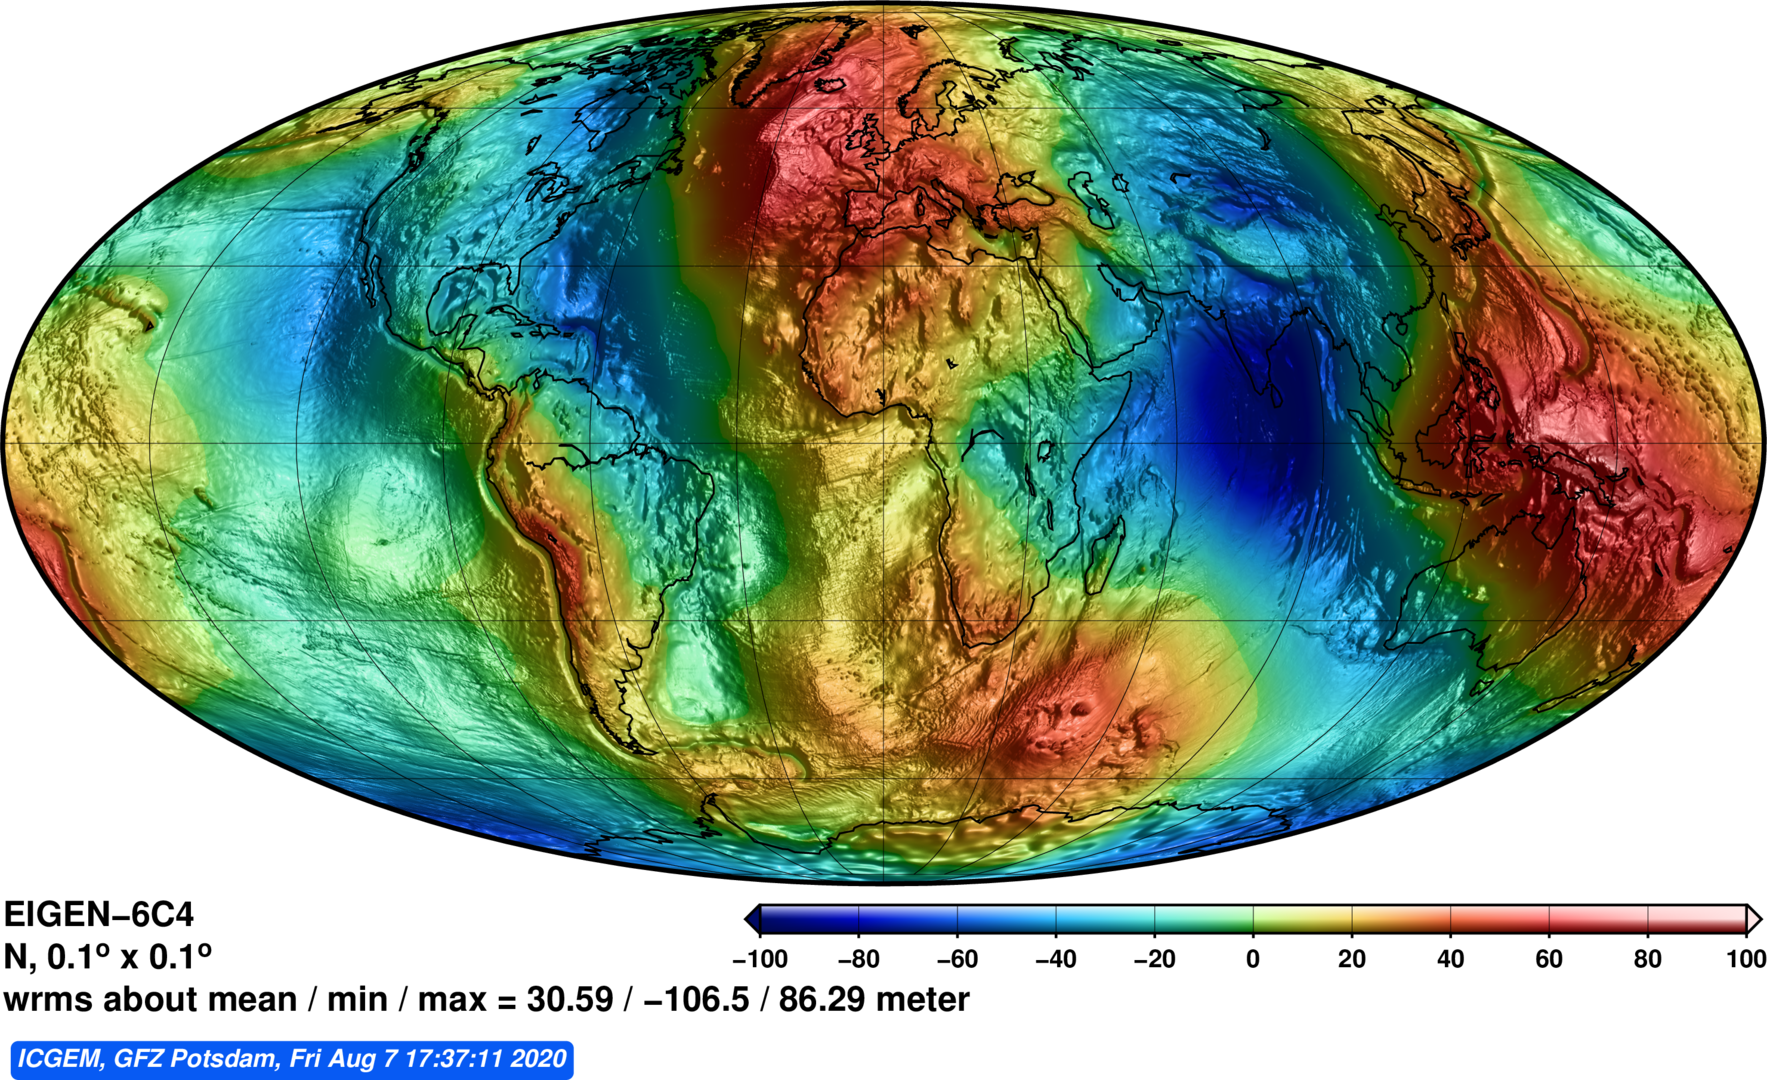
\includegraphics[scale=0.17]{figs/N.png}
	\caption{Ondulação geoidal da Terra. Retirado do \textit{International Centre for Global Earth Models} \href{http://icgem.gfz-potsdam.de/home}{(ICGEM)}.}
	\label{fig:N}
\end{figure}
\FloatBarrier
A ondulação geoidal da Figura \ref{fig:N} representa a distância entre as superfícies do geoide e do elipsoide ao redor do globo, que fica em torno $\pm 100m$ \cite{jekeli2000}. As ondulações do geoide se distribuem pela Terra e podem ser calculadas de acordo com um modelo de ondulação geoidal. Para exemplificar, foi calculado o valor de $N$ para um ponto de observação localizado na portaria do edifício do \textit{Instituto de Geociências da Universidade Federal Fluminense} ($22.90$º$S$, $43.13$º$W$), a partir do \textit{Modelo de Ondulação Geoidal do Brasil} (MAPGEO2015) do \textit{Instituto Brasileiro de Geografia e Estatística} (IBGE). Este é o modelo de ondulação geoidal brasileiro mais recente, e permite calcular $N$ em um ponto ou conjunto de pontos do território brasileiro a partir das suas coordenadas planimétricas. Para mais detalhes acerca da metodologia utilizada neste modelo, o leitor é convidado a \citeonline{mapgeo2015}. Para o ponto em questão, obteve-se uma ondulação de $-6.00$ m. Ou seja, significa que nesta localidade o geoide esta cerca de $6$ m abaixo do elipsoide. A Figura \ref{fig:superficies equipotenciais} esquematiza as principais superfícies e suas respectivas altitudes.

\begin{figure}[H]
	\centering
	\includegraphics[scale=1.2]{figs/s.png}
	\caption{Modelo esquemático das superfícies equipotenciais, altitudes geométrica ($h$) e ortométrica ($H$) e ondulação geoidal ($N$).}
	\label{fig:superficies equipotenciais}
\end{figure}

\subsection{Anomalia e distúrbio de gravidade}

Considere um ponto $P$ sobre a $SFT$. Projetando-o sobre o geoide e o elipsoide, acompanhando a linha de prumo, são fixados os pontos $Q^{\prime}$ e $Q$, respectivamente, conforme a Figura \ref{fig:disturbio}. O vetor anomalia de gravidade ($\Delta \mathbf{g}_P$) é uma grandeza muito utilizada na geofísica e pode ser definida como sendo a diferença entre $\mathbf{g}_{Q^{\prime}}$ e $\mathbf{\gamma}_{Q}$, ou seja, a diferença entre o vetor gravidade avaliado sobre o geoide (Q') e o vetor gravidade normal no elipsoide (Q).

\begin{equation}
\label{eq:vetor_anomalia de gravidade}
\displaystyle {\Delta \mathbf{g}_P = \mathbf{g}_{Q^{\prime}} - \boldsymbol{\gamma}_Q}.
\end{equation} O vetor distúrbio de gravidade ($\mathbf{\delta g}_P$) por outro lado, mais conhecido na geodésia, é dado por \cite{torge,hofmann2006}:

\begin{equation}
\label{eq:vetor_disturbio}
\displaystyle {\delta \mathbf{g}_P = \mathbf{g}_P - \boldsymbol{\gamma}_P},
\end{equation} e o distúrbio de gravidade é calculado fazendo a diferença entre as equações \ref{eq:gravidade_g} e \ref{eq:gravidade_normal}, de forma que:

\begin{equation}
\label{eq:disturbio}
\displaystyle {\delta g_P = \parallel\mathbf{g}_P\parallel - \parallel\boldsymbol{\gamma}_P\parallel}.
\end{equation}

\begin{figure}[H]
	\centering
	\includegraphics[scale=0.5]{figs/disturbio_de_gravidade.png}
	\caption{Representação esquemática dos vetores de gravidade em um ponto $P$ sobre a superfície física da Terra.	$\mathbf{g}_P$ é o vetor gravidade, $\gamma_{P}$ é o vetor de gravidade normal, $\delta g_{P}$ é o vetor de distúrbio de gravidade, $\mathbf{\hat{u}}_{P}$ é vetor unitário da equação \ref{eq:vetores_unitarios}, $g_{Q}$ é o vetor de gravidade em um ponto ${Q'}$ sobre o geoide, $\gamma_{Q}$ é o vetor de gravidade normal em um ponto ${Q}$ sobre o elipsoide, $h_{P}$ é a altitude geométrica, $H_{P}$ é a altitude ortométrica e $N_{P}$ é a ondulação geoidal associadas ao ponto ${P}$. Os pontos ${P}$ e ${Q}$ possuem as mesmas latitude e longitude. A linha pontilhada $\overline{PQ}$ é \textit{normal} ao elipsoide de referência e representa a linha de campo associada ao campo de gravidade normal. Retirado de \citeonline{kristoffer}}.
	\label{fig:disturbio}
\end{figure}

 

A diferença entre o potencial de gravidade da Terra Real ($W$) e o potencial de gravidade da Terra Normal ($U$), no mesmo ponto $P$, fornece o potencial anômalo ou perturbador $T$ \cite{escobar2000,hofmann2006} 

\begin{equation} \label{eq:potencial_anomalo}
\begin{gathered}
\displaystyle {T_{P} = W_{P} - U_{P}} \\
\displaystyle {T_{P} = V_{P} - \tilde{V_{P}} }.
\end{gathered}
\end{equation} Substituindo as equações~\ref{eq:integral_potencial_gravitacional} e \ref{eq:integral_potencial_gravitacional_normal} em \ref{eq:potencial_anomalo}, verifica-se que $T$ é produzido pela distribuição de massas anômalas $(\Delta \rho)$,

\begin{equation} \label{eq:massas_anomalas}
\displaystyle { T = G \int_{v_0} \frac{\Delta \rho dv'}{| \mathbf{r} - \mathbf{r'} |} }
\end{equation} em que $v_{0}$ é a diferença entre Terra Real e Terra normal, $\Delta \rho = \rho - \tilde{\rho}$. Por se tratar do mesmo ponto, $T$ independe de $\Phi$ e seu efeito é puramente gravitacional, satisfazendo a equação \ref{eq:laplaciano}, ou seja, $T$ é um potencial harmônico \cite{lopes2006}.

Levando em conta as relações~\ref{eq:vetor_gravidade_g} e \ref{eq:vec_gravidade_normal}, conclui-se que $\delta \mathbf{g}_P$ é o \textit{gradiente} do potencial perturbador $T$  \cite{heiskanen1967,hofmann2006}:

\begin{equation} \label{eq:disturbio de gravidade=potencial anomalo}
\begin{gathered}
\displaystyle {\mathbf{\delta g}_{P} = \mathbf{\nabla} W_{P}-\mathbf{\nabla} U_{P}} \\
\displaystyle {\mathbf{\delta g}_{P} = \mathbf{\nabla} T_{P}}.
\end{gathered}
\end{equation} 

É imprescindível enfatizar que a anomalia de gravidade no ponto $P$ sobre a $SFT$ é calculada usando a gravidade sobre o geoide e a gravidade normal sobre o elipsoide. Desta forma, a remoção da parte centrífuga do dado não é realizada em sua totalidade. A anomalia de gravidade continua apresentando o resultado da combinação linear de efeitos gravitacionais e centrífugos, mesmo que em menor escala. Ela é amplamente utilizada como dado de entrada em vários estudos na literatura e é comumente associada ao potencial perturbador por meio da aproximação conhecida pela equação fundamental da geodésia \cite{arana2009}. Sob o aspecto da teoria do potencial e segundo os argumentos apresentados, o distúrbio de gravidade é a grandeza mais acurada para ser aplicada pois avalia $g$ e $\gamma$ no mesmo ponto P conforme mostrado na Figura \ref{fig:disturbio}. Para efeito de comparação, as Figuras \ref{subfig:anomalia}.a e b exemplificam a anomalia e distúrbio de gravidade, respectivamente, sobre a América do Sul. A Figura \ref{subfig:anomalia}.c apresenta o mapa de diferença entre distúrbio e anomalia de gravidade. Pode-se constatar que as principais diferenças se encontram na região dos Andes (valores positivos) e na porção Norte da América do Sul (valores negativos). Adicionalmente, pode-se verificar algumas disformidades de valores negativos na porção continental brasileira. Além disso, nota-se similaridades das componentes de longo comprimento de onda entre o mapa de diferenças e o da ondulação, conforme apresentado na Figura \ref{subfig:anomalia}.d.

\begin{figure}[H]
	\centering
	\subfloat[]{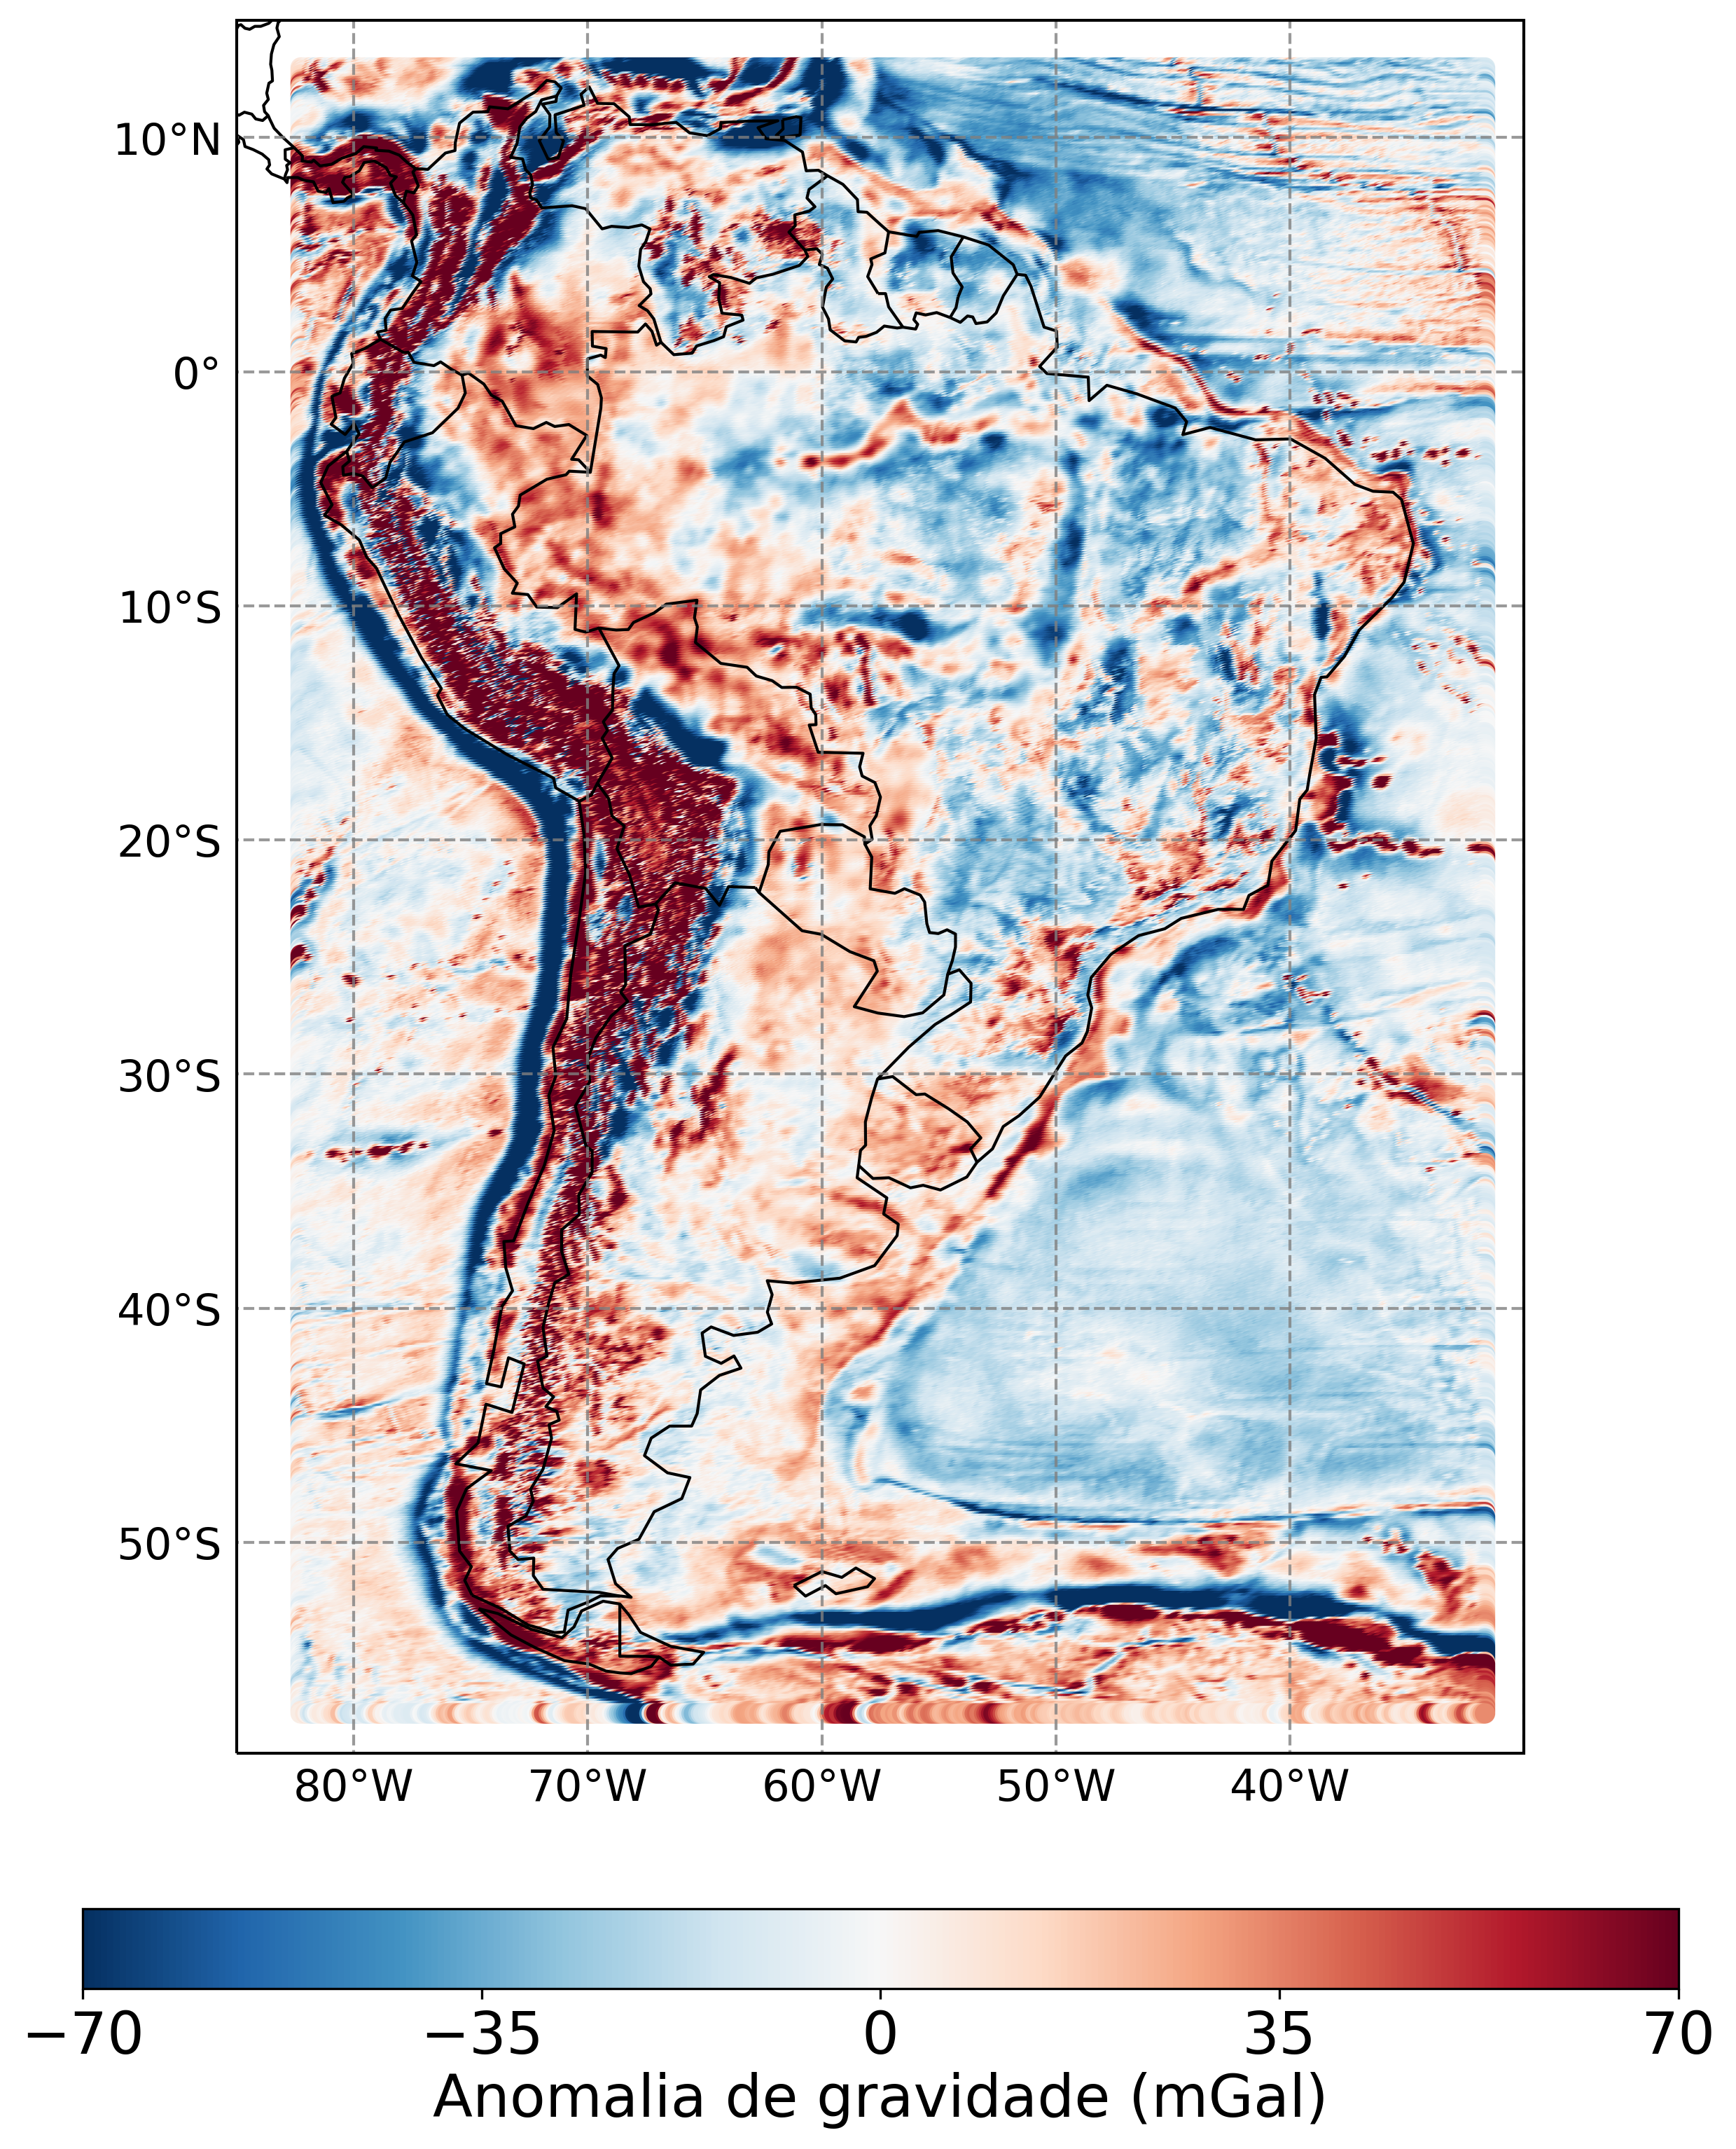
\includegraphics[scale=0.36]{figs/anom_AS.png}}
	\qquad
	\subfloat[]{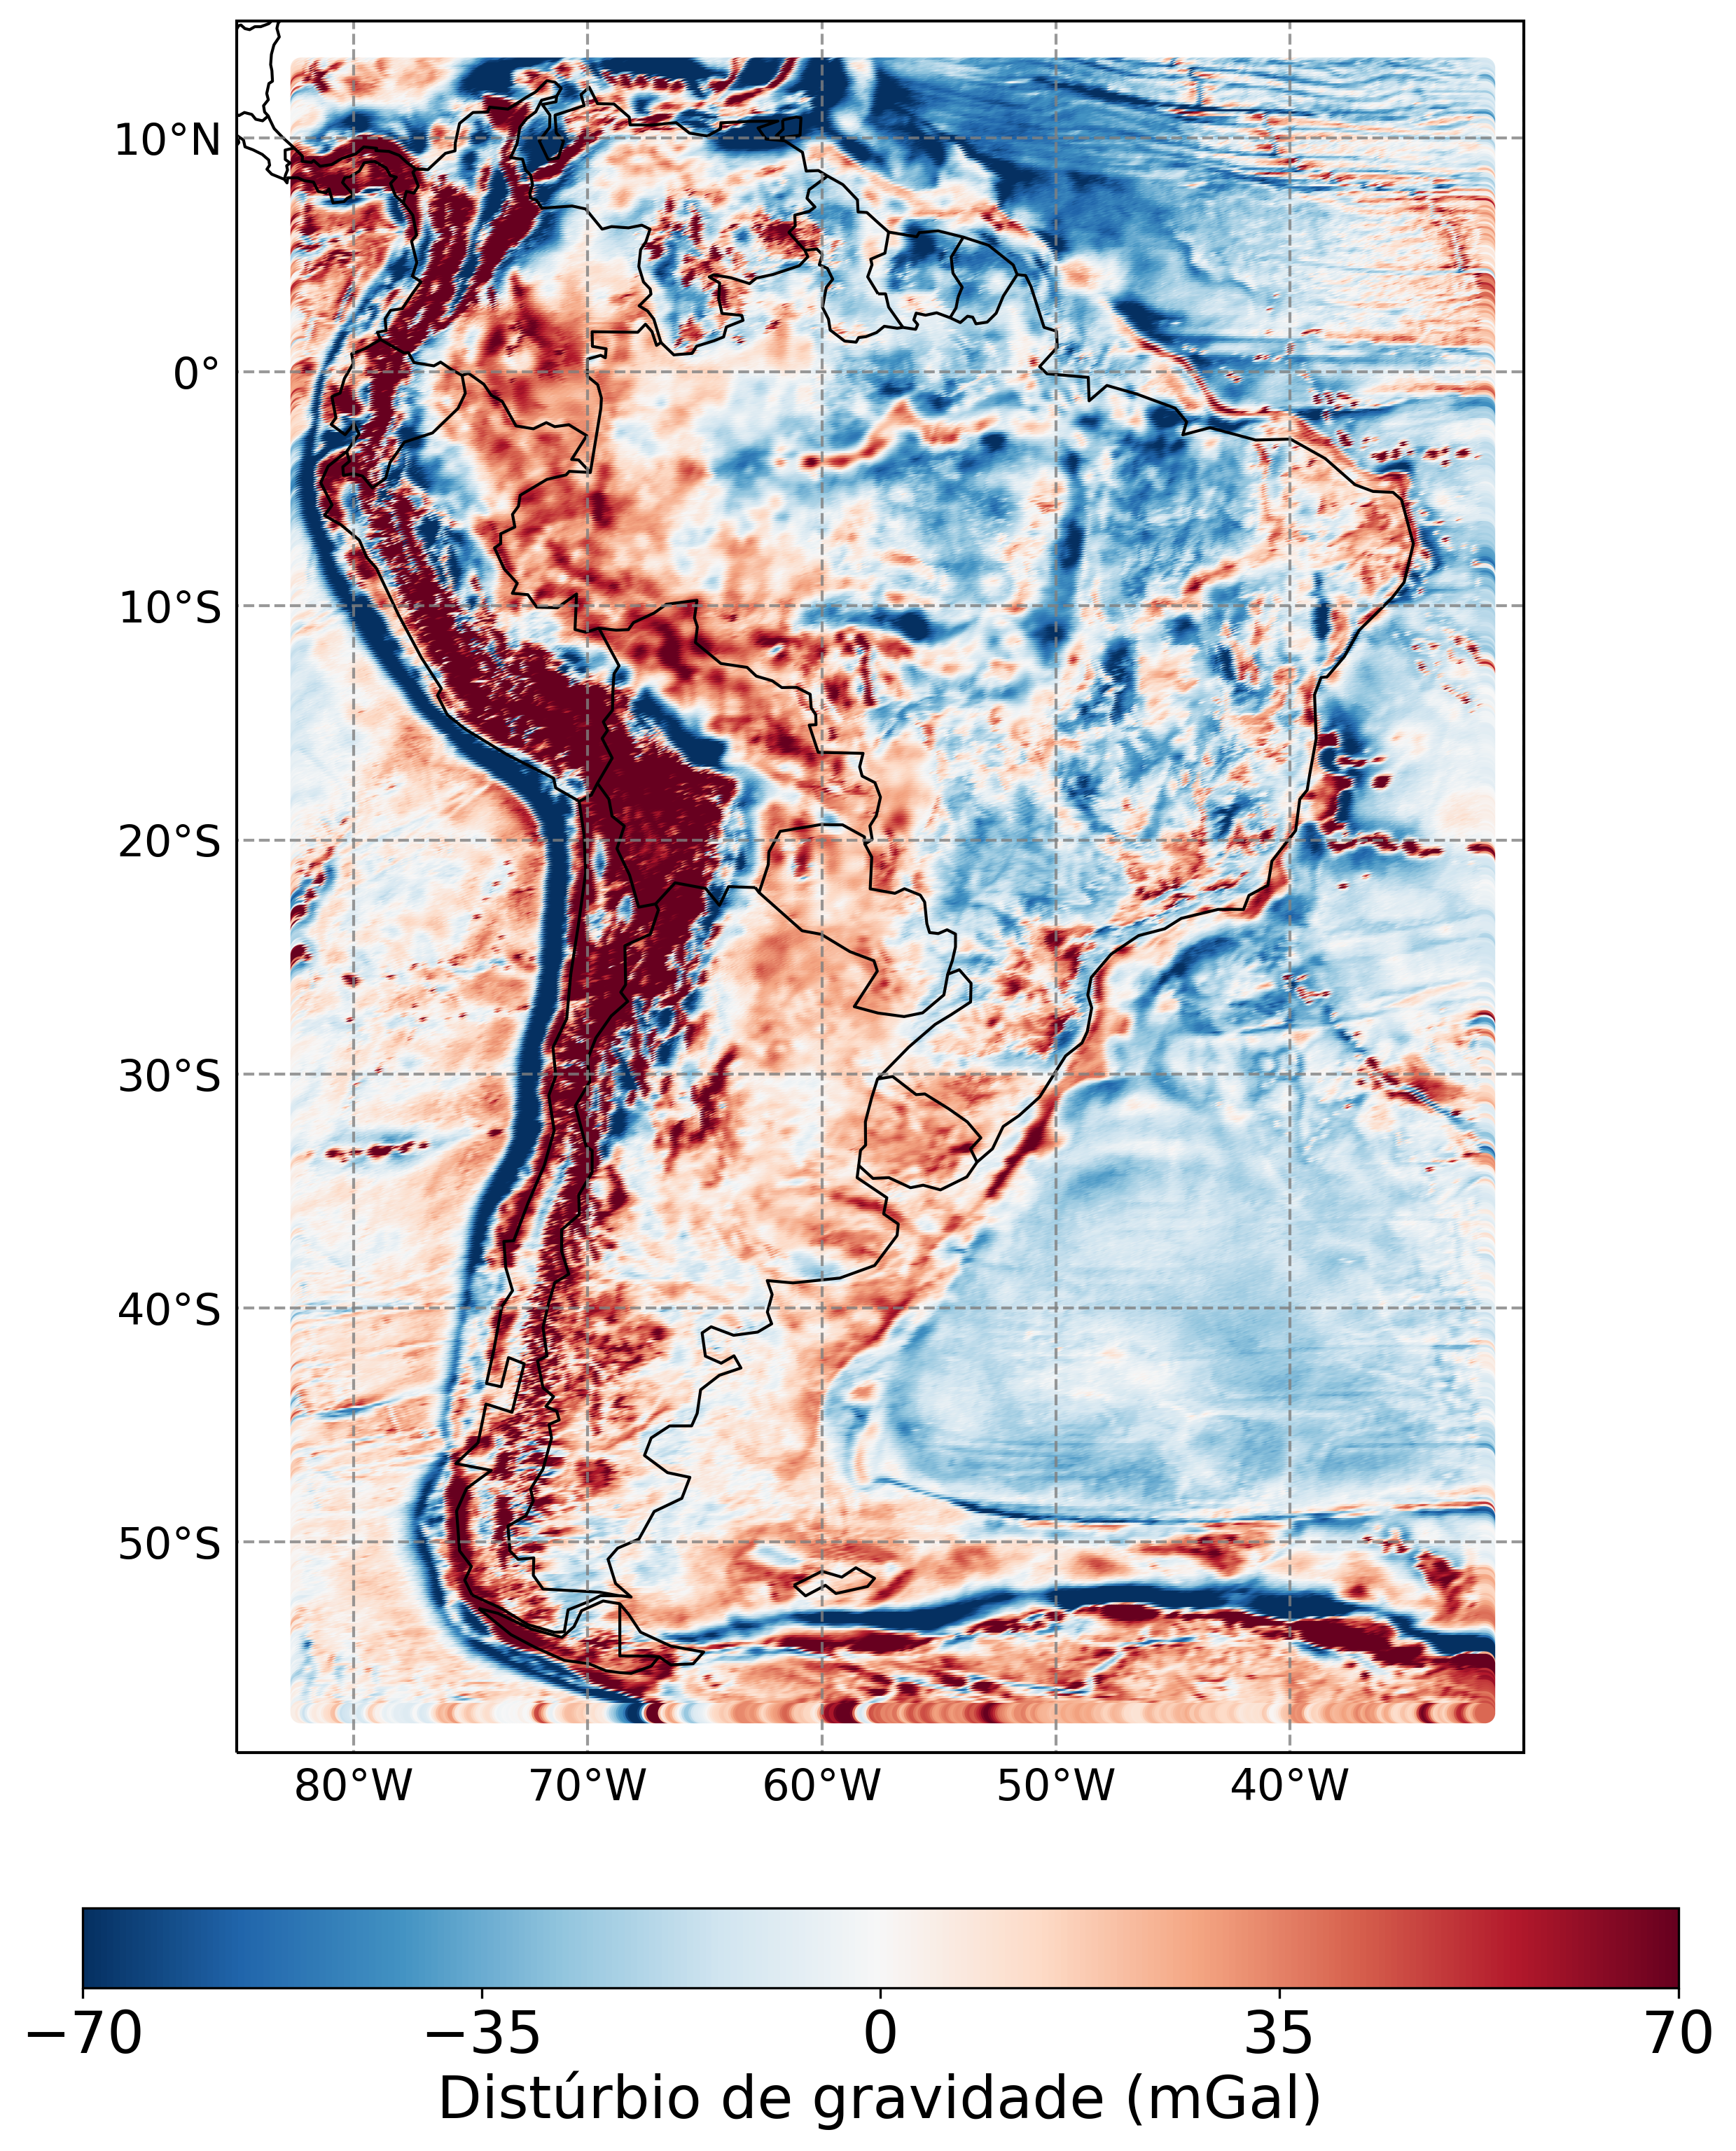
\includegraphics[scale=0.36]{figs/delta_AS.png}}
	\qquad
	\subfloat[]{\includegraphics[scale=0.36]{figs/R_AS.png}}
	\qquad
	\subfloat[]{\includegraphics[scale=0.36]{figs/N_AS.png}}
	\caption{Mapas da anomalia de gravidade (a), distúrbio de gravidade (b), diferença entre distúrbio e anomalia de gravidade (c) e ondulação geoidal (d) sobre a América do Sul. Os contornos pretos representam os limites dos países.}  
	\label{subfig:anomalia}
\end{figure}

% ------------------- capitulo 3:
\chapter{Metodologia}
Um dos objetivos deste estudo é estabelecer uma metodologia para comparar os distúrbios de gravidade de um ponto ou conjunto de pontos, a partir de um MGG. Dessa forma, definimos uma estratégia na qual alguns elementos do campo de gravidade predito pelo modelo de harmônicos esféricos são comparados com os mesmos elementos observados \textit{in situ}. Por conseguinte, é possível analisar a viabilidade desta metodologia em relação à acurácia das estimativas. Para esta avaliação foram utilizados conjuntos de dados de gravimetria e altimetria.

\section{Área de estudo}

A área onde o levantamento terrestre foi realizado corta longitudinalmente a Bacia do Parnaíba (Figura \ref{fig:bacia do parnaiba}). Este estudo produzido pela equipe de geofísica do \textit{Observatório Nacional} (ON) em parceria com a \textit{British Petroleum} (BP) serviu de base para o desenvolvimento deste trabalho, possibilitando confrontar dados terrestres com os dados obtidos via MGG.

\begin{figure}[h]
	\centering
	\includegraphics[scale=0.25]{figs/bacia do parnaiba.png}
	\caption{Mapa da região da Bacia do Parnaíba, em vermelho o perfil das estações onde foram adquiridos os dados terrestres.}
	\label{fig:bacia do parnaiba}
\end{figure}

A bacia do Parnaíba está localizada na região nordeste brasileira, na sua porção ocidental e em partes de áreas vizinhas, distribuindo-se pelos estados do Ceará, Bahia, Piauí, Maranhão, Tocantins e Pará, abrangendo uma área de cerca de $660.000km^{2}$ \cite{article_parnaiba}. É classificada como uma bacia intracratônica, um tipo  comumente localizado em crosta continental estável e espessa, mas relativamente fina se comparada à sua extensão e geralmente com formação associada à separação de supercontinentes em processos de subsidência termal ao longo de sua formação \cite{vaz2007_parnaiba}. Comumente, bacias sedimentares com este histórico são divididas em várias megassequências que podem ter sido formadas em diferentes épocas sob regimes tectônicos distintos. Logo, é necessária uma análise cuidadosa das diferentes fases de formação da bacia \cite{bacias_intracratonicas}. Ainda assim, a morfologia destas bacias está associada, em geral, a um mecanismo tectônico primário, restringindo os mecanismos secundários a modificações menores \cite{allen2012cratonic}. A Bacia do Parnaíba desenvolveu-se sobre embasamento continental durante a estabilização da Plataforma Sul-Americana, e, por correlação com rochas existentes nas faixas de dobramentos, maciços medianos e outras entidades complexas situadas nas bordas ou proximidades da bacia, deduz-se que o seu substrato é formado de rochas metamórficas, ígneas e sedimentares, cujas idades abrangem um intervalo do Arqueano ao Ordoviciano \cite{tese_bacia_parnaiba}. A estrutura geológica define a topografia da região com regiões planas entre os vales, com altitudes de  $\approx 800$m, sendo as cotas maiores localizadas preferencialmente na borda leste onde se localiza uma feição de Serra. 

\section{Descrição dos dados}

\subsection{Gravimetria terrestre}

O levantamento de campo realizado pela equipe de Geofísica do ON percorreu aproximadamente 1200km, iniciando na margem leste da bacia, no estado do Ceará e finalizando na margem oeste, no estado do Pará. O perfil traçado em vermelho no mapa da Figura \ref{fig:bacia do parnaiba} corresponde ao caminho feito durante o levantamento, cujo objetivo original era realizar um levantamento gravimétrico terrestre cortando a bacia do Parnaíba de leste a oeste.

O gravímetro diferencial Autograv-CG5 da Scintrex (Figura \ref{subfig:gravimetro-gps}.a) e o receptor GNSS da Trimble (Figura \ref{subfig:gravimetro-gps}.b), foram os equipamentos utilizados para medir a gravidade e as coordenadas plani-altimétricas ao longo de todo o levantamento, respectivamente. O gravímetro diferencial é um equipamento bastante comum em levantamentos de campo devido a suas características técnicas e simplicidade de operação \cite{cg5} e com precisão da ordem de 1$\mu$Gal \cite{on_cg5}. Por si só, ele não é capaz de medir a gravidade absoluta, já que a sua leitura consiste em medir a diferença entre estações adjacentes. Consequentemente, a conexão das estações do perfil com pelo menos uma estação de uma rede gravimétrica conhecida, se faz obrigatória. Apesar do equipamento possuir uma antena de GPS própria, esta é somente usada para sincronizar o relógio interno com a hora precisa da constelação de satélites. Isso permite ao gravímetro realizar algumas reduções gravimétricas de forma automática, como as reduções de deriva instrumental (i.e., devido ao desgaste do equipamento) e de maré (i.e., fruto da interferência luni-solar) \cite{geodesia}. É também possível configurar o gravímetro para aplicar reduções de terreno ao dado, porém esse não fora aplicado. O GPS do gravímetro não contém a precisão necessária para determinar as coordenadas planimétricas e também não é capaz de mensurar a altitude geométrica do ponto. Dessa forma, o receptor diferencial da Trimble, cujas coordenadas plani-altimétricas são observadas com precisão centimétrica \cite{trimble,gps}, foi o utilizado nesta expedição. Neste caso, um receptor chamado base é fincado em um local confiável e remoto, livre de interferências, normalmente afastado das estações gravimétricas que caracterizam o levantamento, para ter comunicação direta com a constelação de satélites. Um outro receptor denominado móvel realiza as medidas das coordenadas plani-altimétricas das estações gravimétricas do levantamento. O tempo de exposição e comunicação entre os receptores são essenciais para a obtenção das coordenadas com alta precisão. A tabela \ref{tab:dados_terrestre} resume brevemente a gravimetria e altimetria observadas em campo.

\begin{table}[h]
	\centering
	\caption{Resumo dos dados observados.} \label{tab:dados_terrestre}
	\begin{tabular}{c|c|c|c|c}
		
		Dados & Mínimo & Máximo  \\ 
		\hline                               % para uma linha horizontal
		Latitude (º) & 4,8ºS & 6,35ºS \\
		Longitude (º) & 39,91ºW & 49,28ºW \\
		Gravidade absoluta (mGal) & 977893.4 & 978048.18 \\
		Altitude geométrica (m) & 74,54 & 718,83
		% não é preciso quebrar a última linha	
	\end{tabular}
\end{table}

\begin{figure}[!ht]
	\centering
	\subfloat[Gravímetro relativo \textit{Autograv CG-5} da \textit{Scintrex Ltda.}.]{\includegraphics[width=5cm,height=5cm]{figs/cg5.jpg}}
	\qquad
	\subfloat[Aquisição terrestre com o \textit{Autograv-CG5 } junto ao \textit{GPS Trimble} utilizado para mensurar as coordenadas plani-altimétricas. Retirado de: \textit{Topocart}.]{\includegraphics[width=5cm,height=5cm]{figs/2b}}
	\caption{Equipamentos necessários para realizar um levantamento gravimétrico terrestre.}  
	\label{subfig:gravimetro-gps}
\end{figure}

\subsection{Gravimetria por satélite}

O conjunto de dados de satélite é de domínio público e está disponibilizado no site do ICGEM. Dentro do banco de dados do $ICGEM$, há uma série de modelos que calculam elementos da gravidade. Dentre eles, foi utilizado o modelo \textit{EIGEN-6C4}. Este foi escolhido por se tratar do modelo de gravidade global que possui expansão em harmônicos esféricos de maior grau e ordem, iguais a 2190 \cite{eigen}, em comparação com outros existentes. Trata-se do maior truncamento proposto e que, portanto, melhor representa os sinais de alta frequência contidas nos dados de gravidade.Deste modelo, foram utilizados os funcionais \textit{gravity\_earth} e \textit{gravity} associados às malhas regulares e estações terrestres, respectivamente, compondo o conjunto de dados preditos.
\subparagraph{Funcional \textit{gravity$\_$earth}:} De acordo com \citeonline{barthelmes2009}, o funcional \textit{gravity\_earth}, selecionado pela aba \textit{Regular grids}, aplica a técnica de expansão em harmônicos esféricos ao potencial de gravidade, para calcular a gravidade absoluta sobre a $SFT$, sendo esta a magnitude do gradiente de $W$ (equação \ref{eq:vetor_gravidade_g}) nas respectivas coordenadas planimétricas escolhidas pelo usuário. Para mais detalhes acerca dessa aplicação, o leitor é convidado à \citeonline{barthelmes2009}. As malhas regulares de satélite abrangem uma área definida pelas latitudes $0.2$º$S$ $\leq \varphi \leq$ $11.78$º$S$ e longitudes $39.5$º$W$ $\leq \lambda \leq$ $50$º$W$, ambas em graus decimais e com espaçamento de $0.03$º. A escolha dos limites $\varphi$ e $\lambda$ está relacionada com a localização da Bacia do Parnaíba, que consta como o alvo do estudo. Estas malhas serviram para analisar a bacia sob uma ótica regional. O espaçamento possibilitou uma amostragem maior, com $135837$ pontos analisados. Este funcional gera um arquivo com as seguintes colunas: longitude e latitude em graus decimais; as altitudes ortométricas em metros de cada ponto definido pelo usuário; a gravidade absoluta em mGal. A tabela \ref*{tab:dados_sat} resume brevemente o conjunto de dados calculados pelo funcional \textit{gravity\_earth}. A variação entre o maior e o menor valor da gravidade absoluta obtida foi de $373$ $mGal$, enquanto as altitudes ortométricas tiveram uma variação de $1322.92$m. 

\begin{table}[h]
	\centering
	\caption{Resumo dos dados calculados pelo funcional \textit{gravity\_earth}.} 
	\label{tab:dados_sat}
	\begin{tabular}{c|c|c|c|c}
		
		Dados & Mínimo & Máximo  \\ % Note a separação de col. e a quebra de linhas
		\hline                               % para uma linha horizontal
		Latitude (º) & 0,2ºS & 11,78ºS \\
		Longitude (º) & 39,5ºW & 50ºW \\
		Gravidade absoluta (mGal) & 977811.88 & 978184.24 \\
		Altitude ortométrica (m) & 0 & 1322.92
		% não é preciso quebrar a última linha	
	\end{tabular}
\end{table}
\subparagraph{Funcional \textit{gravity}:} O funcional \textit{gravity}, selecionado na aba \textit{User-defined points}, calcula, por meio da expansão em harmônicos esféricos, a gravidade absoluta como sendo a magnitude do vetor gravidade, ou seja, o módulo do gradiente de $W$, para quaisquer conjuntos de pontos de observação $(h, \varphi,\lambda)$ definidos pelo usuário \cite{barthelmes2009}. Para o cálculo através deste funcional, foram inseridas as coordenadas plani-altimétricas referentes às estações do levantamento terrestre, sobre as quais foram calculadas os respectivos valores de gravidade absoluta. Este funcional gera um arquivo com as seguintes colunas: longitude e latitude em graus decimais; as altitudes geométricas em metros de cada ponto definido pelo usuário; a gravidade em $mGal$ calculada sobre as coordenadas correspondentes. A tabela \ref{tab:dados_sat_pred} mostra as informações pertinentes a estes dados. Observa-se uma variação de $152$ $mGal$ entre os valores máximo e mínimo de gravidade absoluta e de aproximadamente $644$m nas altitudes geométricas observadas. 

\begin{table}[H]
	\centering
	\caption{Resumo dos dados calculados pelo funcional \textit{gravity}.}
	\label{tab:dados_sat_pred}
	\begin{tabular}{c|c|c|c|c}
		
		Dados & Mínimo & Máximo  \\ % Note a separação de col. e a quebra de linhas
		\hline                               % para uma linha horizontal
		Latitude (º) & 4,8ºS & 6,35ºS \\
		Longitude (º) & 39,91ºW & 49,28ºW \\
		Gravidade absoluta (mGal) & 977877.06 & 978029.54 \\
		Altitude geométrica (m) & 74,54 & 718,83 
		% não é preciso quebrar a última linha	
	\end{tabular}
\end{table}

\subsection{Altimetria por satélite}
O conjunto de dados disponibilizados na plataforma do $ICGEM$ não se restringem exclusivamente a elementos da gravidade. Dentre os funcionais disponíveis, também é possível calcular a topografia para qualquer região do globo. Portanto, foi adicionada ao estudo uma análise para comparar as altitudes  geométricas calculadas pelo modelo com as altitudes geométricas observadas. 
\subparagraph{Funcional \textit{h\_topo\_over\_ell}:} Este funcional é selecionado, assim como o \textit{gravity}, na aba \textit{User-defined points}. Ele calcula a altura da topografia sobre o elipsoide (i.e., a distância entre um ponto na $SFT$ e o elipsoide de referência), para um ponto ou conjunto de pontos informados pelo usuário. Este cálculo é feito por interpolação bilinear entre o modelo de elevação, relacionado ao geoide, somado a $N$. Este funcional gera um arquivo com as seguintes colunas: longitude e latitude em graus decimais; as altitudes geométricas em metros, calculadas através dos harmônicos esféricos. A tabela \ref{tab:dados_h_pred} mostra as informações pertinentes a estes dados. É importante ressaltar que as altitudes preditas por este funcional não foram utilizadas para o cálculo dos distúrbios de gravidade, detalhados na seção \ref{subsec:delta}, onde foram utilizadas as altitudes observadas. 

\begin{table}[H]
	\centering
	\caption{Resumo dos dados calculados pelo funcional \textit{h\_topo\_over\_ell}.}
	\label{tab:dados_h_pred}
	\begin{tabular}{c|c|c}
		
		Dados & Mínimo & Máximo  \\ % Note a separação de col. e a quebra de linhas
		\hline                               % para uma linha horizontal
		Latitude (º) & 4,8ºS & 6,35ºS \\
		Longitude (º) & 39,91ºW & 49,28ºW \\
		Altitude geométrica (m) & 48,14 & 681,26
		% não é preciso quebrar a última linha	
	\end{tabular}
\end{table}

\section{Cálculo da altitude geométrica ($h$) e do distúrbio de gravidade ($\delta g$)}

Todos os cálculos foram realizados em linguagem Python utilizando os dados descritos anteriormente. Os distúrbios de gravidade foram obtidos de acordo com a equação \ref{eq:disturbio}, seguindo o fluxograma de trabalho descrito na Figura \ref{fig:fluxograma}.

\begin{figure}[H]
	\centering
	\includegraphics[scale=0.45]{figs/flux_novo.png}
	\caption{Fluxograma de trabalho adotado ao longo do desenvolvimento deste estudo.}
	\label{fig:fluxograma}
\end{figure} 

\subsection{Altitude geométrica (h)}

Como discutido no capitulo sobre fundamentação teórica, o cálculo do distúrbio de gravidade requer o conhecimento da gravidade normal. Com o efeito, a altitude geométrica é uma grandeza indispensável para que os distúrbios sejam calculados adequadamente.
 
Como descrito na seção anterior, o funcional \textit{gravity\_earth} fornece os valores de gravidade e de altitude ortométrica. Portanto, para obter as altitudes geométricas deste conjunto de pontos sobre a $SFT$ foi necessário calcular os valores de ondulação geoidal $N$. A informação referente à ondulação geoidal dos pontos de observação foi adquirida por intermédio do programa \textit{MAPGEO2015}, disponibilizado pelo site do \href{https://www.ibge.gov.br/geociencias/modelos-digitais-de-superficie/modelos-digitais-de-superficie/10855-modelo-de-ondulacao-geoidal.html?=&t=o-que-e}{IBGE}, que representa o modelo aproximado de $N$ mais recente do Brasil. Os valores de $N$, em metros, de um ponto ou conjunto
de pontos são calculados a partir das coordenadas planimétricas \cite{mapgeo2015}. De posse das altitudes ortométricas e das ondulações geoidais de cada ponto da malha regular, as altitudes geométricas puderam ser calculadas por meio da equação \ref{eq:geometric}. A Figura \ref{fig:altitude geometrica grid} mostra o mapa da malha regular referente à altitude geométrica da região da bacia do Parnaíba. É importante destacar que $H$ e $N$ foram calculados em sistemas de referências diferentes, \textit{WGS84} e \textit{SIRGAS2000}, respectivamente. No entanto, são sistemas de referência análogos e este processo não precisou ser feito para o restante dos dados, já que as medidas de campo fornecem os valores de altitude geométrica para cada estação.

\begin{figure}[H]
	\centering
	\includegraphics[scale=0.32]{figs/altitude geometrica da bacia do parnaiba.png}
	\caption{Altitude geométrica da região da bacia do Parnaíba, gerada com valores $h$ calculados a partir dos dados de $H$ do funcional \textit{gravity\_earth} e $N$ do \textit{MAPGEO2015} através da equação \ref{eq:geometric}. A região contornada em preto representa os limites da Bacia do Parnaíba e apresentou uma variação de cerca de $1309$ metros. Os contornos em cinza pontilhados representam o contorno dos estados.}	
	\label{fig:altitude geometrica grid}
\end{figure}

\subsection{Distúrbio de gravidade}
\label{subsec:delta}
Os distúrbios de gravidade foram calculados de acordo com a equação \ref{eq:disturbio}, tanto para a malha regular quanto para as estações gravimétricas terrestres. Para tal, foram utilizados os funcionais do ICGEM \textit{gravity\_earth} (para a malha) e o \textit{gravity} (para as estações). A gravidade normal, fundamental para o cálculo de $\delta g$, pode ser calculada de diversas formas. A mais comum é via fórmula internacional da gravidade, que calcula a gravidade normal sobre o elipsoide de referência \cite{somigliana}. No entanto, foi utilizada a fórmula analítica da gravidade proposta por \citeonline{li2001}, pois essa calcula a gravidade normal sobre qualquer ponto fora da Terra Normal (elipsoide). A fórmula analítica utiliza as latitudes geodésicas ($\varphi$) e as altitudes geométricas ($h$) de cada ponto analisado. Os mapas da Figura \ref{subfig:disturbio}.a, b e c mostram os dados para a malha regular. A Figura \ref{subfig:disturbio}.a representa a gravidade absoluta calculada sobre a $SFT$. É possível constatar um contraste de gravidade absoluta, principalmente na borda Leste da bacia e na região mais a Centro-Oeste, onde se nota valores mais baixos.  A Figura \ref{subfig:disturbio}.b refere-se a gravidade normal, que mostrou maior sensibilidade à $SFT$, principalmente na borda Leste, onde estão localizadas as maiores elevações da bacia. Este padrão está relacionado ao cálculo através da fórmula analítica da gravidade, que considera a altitude geométrica dos pontos. Se compararmos os mapas de gravidade absoluta e normal, nota-se um padrão homogêneo na região Nordeste no mapa da Figura \ref{subfig:disturbio}.b, que é discrepante do mapa da Figura \ref{subfig:disturbio}.a. Adicionalmente, há uma diferença significativa entre as cores de cada mapa, principalmente na porção central. Isso pode estar relacionado à questões deposicionais da bacia. Por fim, a Figura \ref{subfig:disturbio}.c mostra o distúrbio de gravidade, calculado sobre a $SFT$. É possível inferir que o depocentro da bacia está situado na porção mais ao norte, visto que, essa região apresenta um padrão de distúrbio negativo com altitude geométrica relativamente baixa. Essa conformidade nos leva a crer que a bacia têm um padrão deposicional com orientação $NE$-$SW$ \cite{tese_bacia_parnaiba}. Em sua porção Sul, em torno de ($10.5$ºS;$47$ºW), é notório que os baixos valores de distúrbio de gravidade contrastam com a topografia relativamente alta. Provavelmente, essa não conformidade pode estar associada a heterogeneidades crustais com baixos valores de contraste de densidades.
\begin{figure}[H]
	\centering
	\subfloat[Gravidade absoluta da região da bacia do Parnaíba, calculada a partir do funcional \textit{gravity\_earth}.]{\includegraphics[scale=0.3]{figs/gravidade absoluta da bacia do parnaiba.png}} 
	\
	\subfloat[Gravidade normal da região da bacia do Parnaíba, calculada a partir da fórmula analítica da gravidade.]{\includegraphics[scale=0.3]{figs/gravidade normal da bacia do parnaiba.png}}
	\qquad
	\subfloat[Distúrbio de gravidade da região da bacia do Parnaíba, calculado pela equação \ref{eq:disturbio}.]{\includegraphics[scale=0.3]{figs/disturbio da bacia do parnaiba.png}}
	\caption{Malhas regulares das gravidades absoluta, normal e do distúrbio de gravidade.}  
	\label{subfig:disturbio}
\end{figure}

% ------------------- capitulo 4:
\chapter{Resultados e discussões}

\section{Altitude geométrica ($h$)}

Foram geradas imagens para analisar a altimetria da região da bacia do Parnaíba. A Figura \ref{fig:comparacao_h} compreende a sobreposição das estações gravimétricas do levantamento à malha regular obtida através do modelo \textit{EIGEN-6C4} no fundo da imagem. Ambas retratam $h$, cujos valores estão dentro da escala de cores definida. É possível observar na malha regular um contraste de $h$ que identifica o padrão transicional entre as plataformas continental e oceânica, onde se destacam as maiores elevações nas porções sul e leste da bacia e as menores elevações na porção norte. Através da análise dos padrões observados e preditos é possível constatar boa similaridade entre as diferentes metodologias de aquisição de dados, terrestre e satélites, e nos leva a crer que são correlatas. Contudo, em alguns pontos específicos, os valores de $h$ observados aparentam ter diferenças em comparação com os preditos. Sendo assim, teve-se a necessidade de calculá-las sobre as respectivas estações. Seguindo este raciocínio, a Figura \ref{subfig:residuos_h}.a representa $h$ observado e a Figura \ref{subfig:residuos_h}.b, $h$ predito do levantamento terrestre. É possível constatar uma conformidade geral, no entanto existem incongruências pontuais entre as duas figuras, como na região entre $42$º$W$ e $43.5$º$W$. A diferença entre as altitudes geométricas pode ser vista no mapa da Figura \ref{subfig:residuos_h}.c que corresponde ao resíduo obtido. Este mapa apresenta uma variação de $\pm 62.5$ $m$.

\begin{figure}[H]
	\centering
	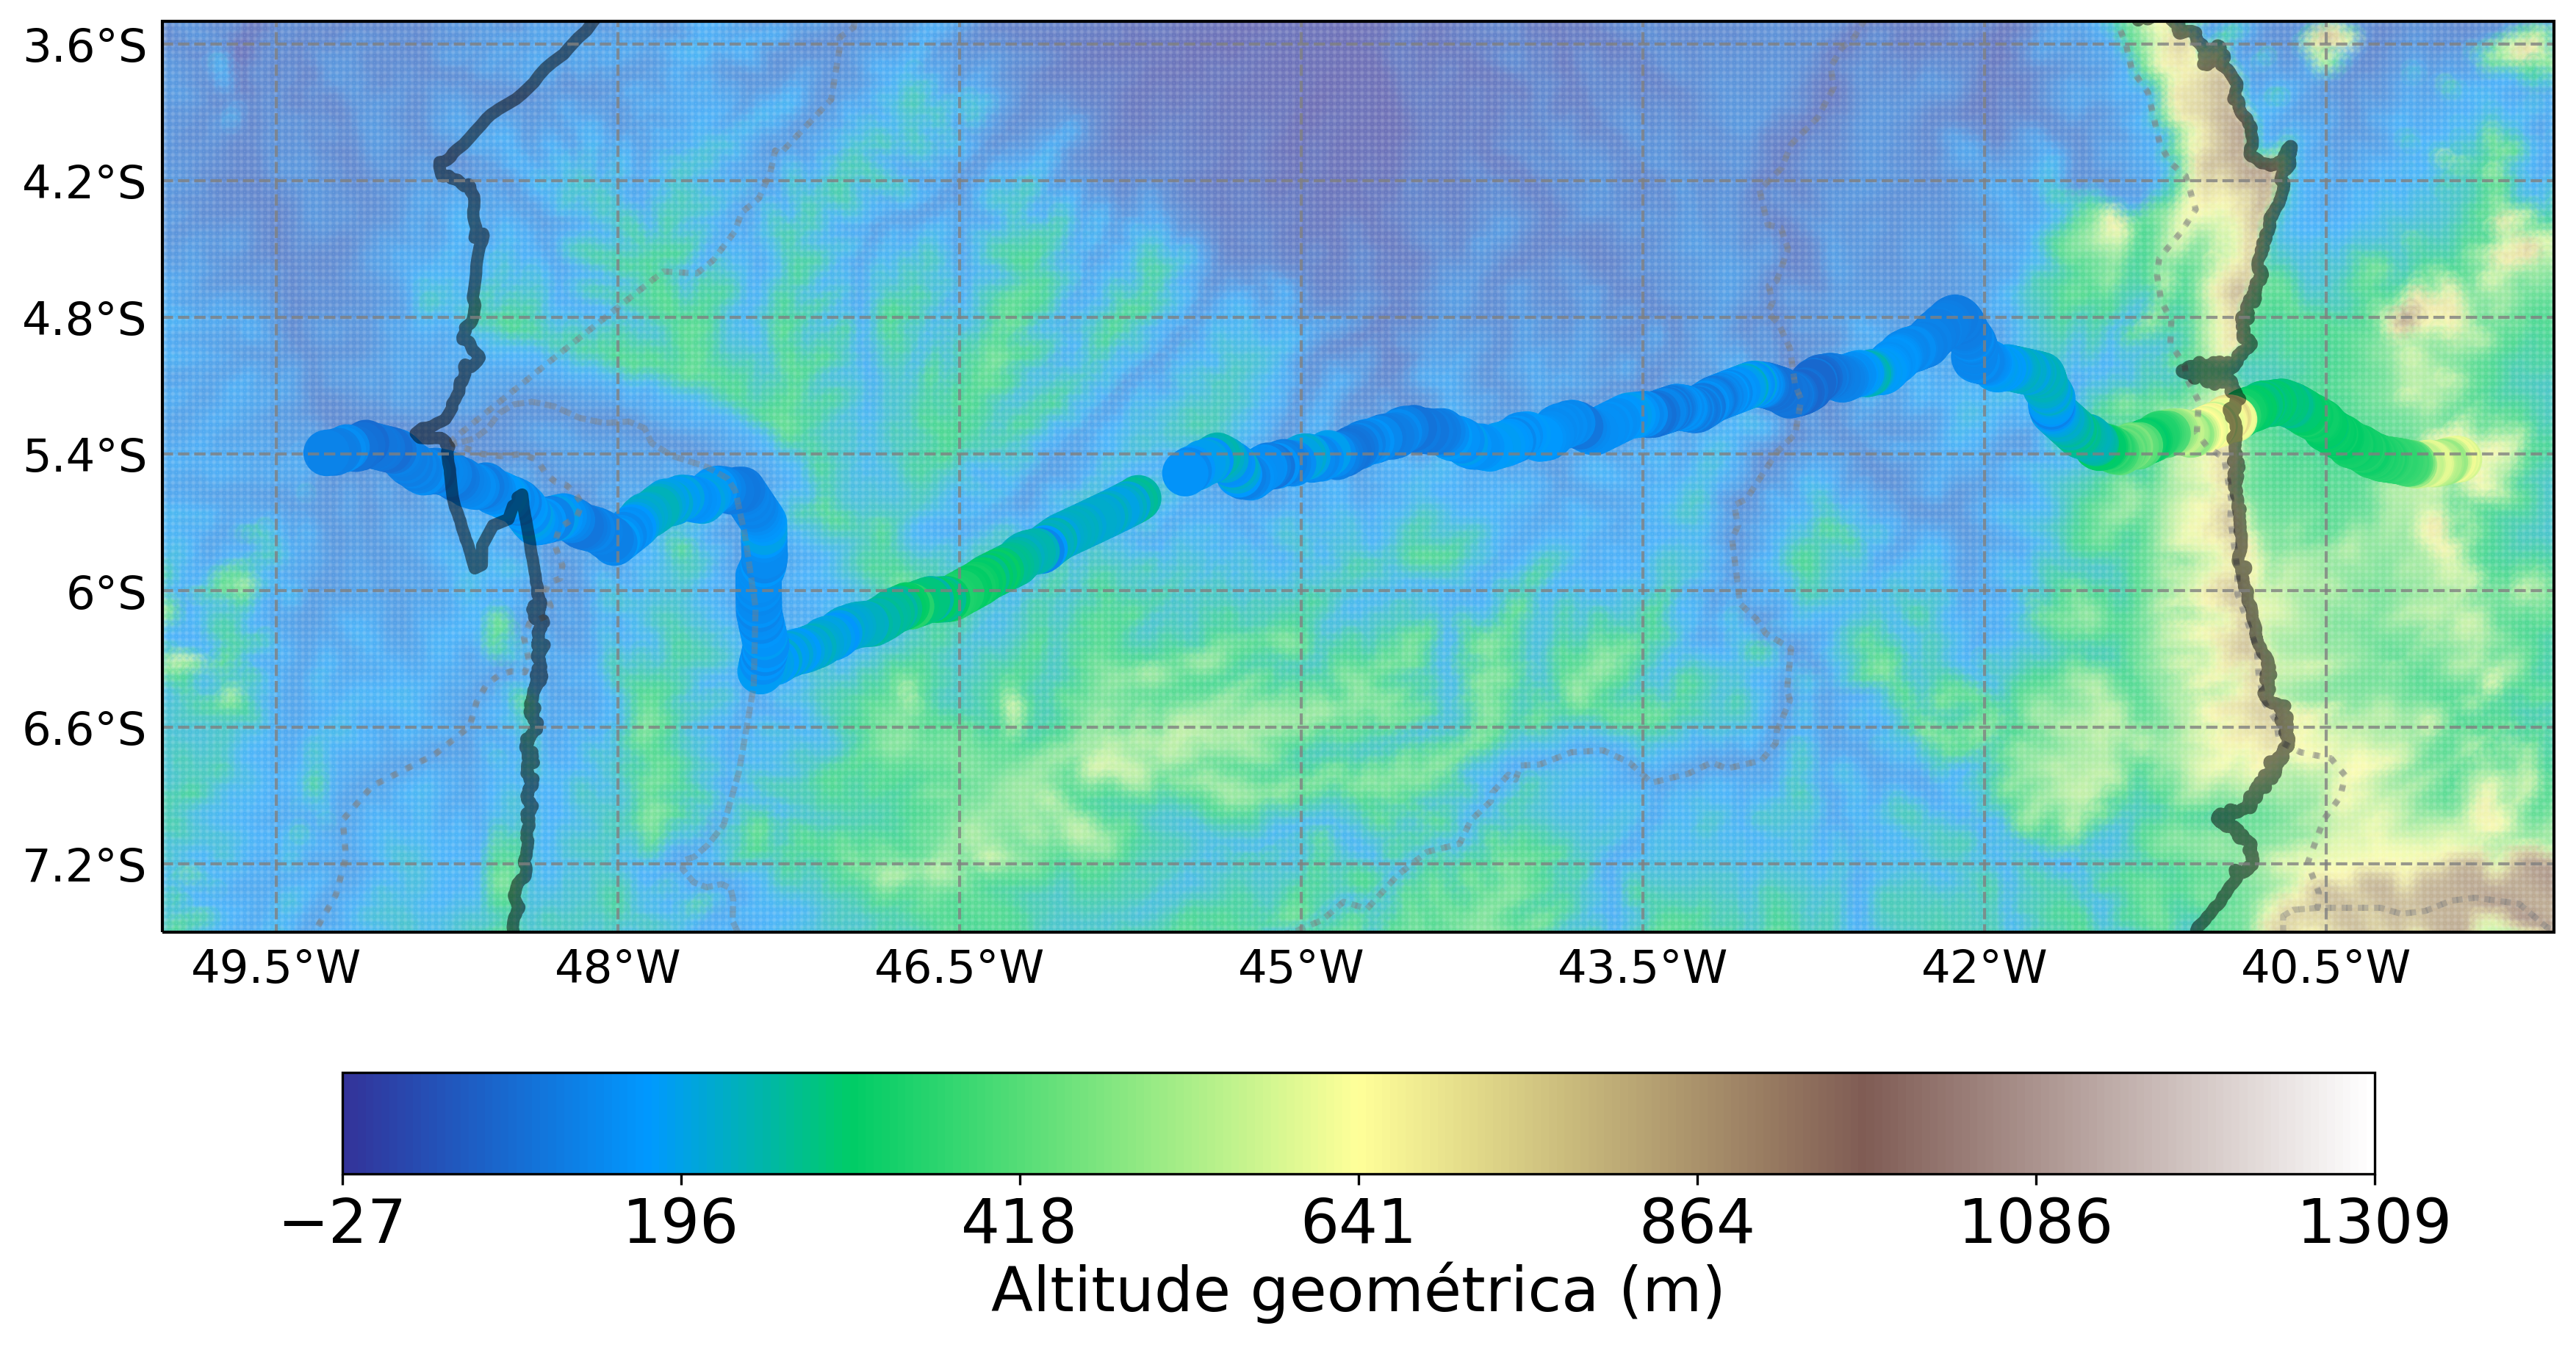
\includegraphics[scale=0.47]{figs/altitude grid x campo.png}	
	\caption{Malha regular da altitude geométrica $h$ da região da Bacia do Parnaíba, sendo o contorno preto os limites da mesma, e o contorno cinza pontilhado, o limite dos estados. Ao fundo temos $h$ predito a partir de $H$ do funcional \textit{gravity earth} e $N$ do \textit{MAPGEO2015}, utilizando a equação \ref{eq:geometric}; sobrepostos, na forma do caminhamento terrestre, estão os valores de $h$ observados. Tanto a malha quanto as estações do levantamento estão sob a mesma escala de cores, variando de $-27$ $m$ a $1309$ $m$.}% É possível observar uma amplitude de até $1309$ metros, e, de uma maneira geral as duas metodologias apresentaram valores muito similares. No entanto, algumas incongruências pontuais entre os pontos e a malha são observados e necessitam de uma melhor análise.}
	\label{fig:comparacao_h}
\end{figure}

\begin{figure}[H]
	\centering
	\subfloat[Mapa com valores de $h$ observados no levantamento terrestre, com variação de $48$ $m$ a $719$ $m$ de acordo com a barra de cores.]{\includegraphics[scale=0.37]{figs/altitude geom campo.png}}
	\qquad
	\subfloat[Mapa com valores de $h$ preditos, pelo funcional \textit{h\_topo\_over\_ell}, apresentando uma variação de $48$ $m$ a $719$ $m$ metros de acordo com a escala de cores.]{\includegraphics[scale=0.37]{figs/altitude geom predita campo.png}}% É possível observar certa similaridade nas altimetrias das diferentes metodologias.]{\includegraphics[scale=0.34]{figs/altitude geom predita campo.png}}
	\qquad
	\subfloat[Mapa de resíduos de $h$, calculados através da diferença entre $h$ observado e predito. com valores variando $\pm62.5$ $m$ segundo a escala de cores.]{\includegraphics[scale=0.37]{figs/residuos altitude geom.png}} %Apresenta uma predominância positiva nos valores dos resíduos, possibilitando inferir que os dados preditos estão subestimados em relação aos dados observados.]{\includegraphics[scale=0.34]{figs/residuos altitude geom.png}}
	\caption{Esquema comparativo de $h$ observado, $h$ predito e os resíduos de $h$ como objeto de comparação. O contorno preto representa os limites da bacia do Parnaíba, e o contorno cinza, o limite dos estados.}  
	\label{subfig:residuos_h}
\end{figure}

Os resíduos de $h$ apresentaram valores majoritariamente positivos, que se repetem com maior frequência  entre as faixas amarela e marrom, segundo a escala de cores, que corresponde à faixa de $0$ à $\approx25$ metros. Essa análise leva à hipótese de que os dados preditos estão subestimados em relação aos observados. É provável que seja resultado do truncamento dos harmônicos esféricos, visto que é necessário impor um trucamento para interromper a expansão em determinado grau e ordem. Para complementar a hipótese da subestimativa de $h$, foi gerado o histograma dos resíduos apresentado na Figura \ref{subfig:histograma_h}.a. Pode-se observar que a média é igual a $17.38$m e desvio padrão de $12.70$m, em que se destaca o comportamento majoritariamente positivo dos resíduos. Essa análise evidencia um erro de tendência. O gráfico de correlação da Figura \ref{subfig:histograma_h}.b entre as altitudes geométricas observadas e preditas apontam para uma região mais densa de pontos para $h$ menor que $400$m, enquanto que para valores mais altos há uma dispersão, aparentemente,  um pouco maior. Isto não prejudica os resultados, já que é possível constatar uma boa correlação linear com o coeficiente de determinação ($R^{2}$) igual à $0.99,$ o que mostra que $h$ predito se ajusta linearmente ao observado com $99$\% de eficácia. No entanto, é preciso levar em conta que a amostragem dos dados tem pouca cobertura em pontos com amplitudes altimétricas maiores. 

\begin{figure}[H]
	\centering
	\subfloat[Histograma dos resíduos de $h$, onde é possível observar um comportamento na média de $17,38$ metros e desvio padrão igual a $12.7$. A linha vermelha pontilhada corresponde ao histograma de resíduo teórico, considerando uma distribuição gaussiana.]{\includegraphics[scale=0.245]{figs/histograma_residuos_h.png}}
	\ 
	\,\,\subfloat[Gráfico de dispersão de $h$, observado e predito, com ajuste linear representado pela reta vermelha com $R^{2}$ igual à $0,99$.]{\includegraphics[scale=0.245]{figs/dispersao h obs x pred.png}}
	\caption{Esquema com histograma de resíduos de $h$ ao lado do gráfico de correlação $h$, observado e predito.}  
	\label{subfig:histograma_h}
\end{figure}


\section{Distúrbio de gravidade ($\delta g$)}

Assim como nas análises altimétricas, foram geradas imagens para analisar $\delta g$ da região da bacia do Parnaíba. A Figura \ref{fig:comparacao_delta} compreende a sobreposição das estações gravimétricas do levantamento à malha regular obtida por satélite no fundo da imagem. Ambas retratam valores de $\delta g$ dentro da escala de cores definida, variando em $\pm70.0$ $mGal$. É possível observar um contraste nos valores de $\delta g$, principalmente na borda leste em relação à porção central, sendo o meio da bacia majoritariamente negativo, fato que já era esperado para uma bacia sedimentar. Destaca-se também que esse padrão tem uma certa correlação com aquele mostrado na Figura \ref{fig:comparacao_h} referente a $h$. Através da análise dos padrões observados e preditos é possível constatar boa similaridade entre as diferentes metodologias de aquisição de dados, terrestre e de satélite. Todavia, nota-se que alguns pontos apresentam valores levemente diferentes de $\delta g$ observados em comparação com os preditos. Sendo assim, foram aplicados os mesmos procedimentos realizados durante a análise de $h$ para $\delta g$. A Figura \ref{subfig:residuos_delta}.a e .b apresenta, para cada estação gravimétrica, os distúrbios observados e preditos, respectivamente. A escala de cores é igual em todos os gráficos, variando em $\pm57$ $mGal$. É possível constatar uma conformidade geral, mas, assim como no caso das altitudes geométricas, existem incongruências pontuais entre os distúrbios, como na região entre $42$º$W$ e $43.5$º$W$, e na região entre $45$º$W$ e $46.5$º$W$. A diferença entre os distúrbios pode ser vista no mapa da Figura \ref{subfig:residuos_delta}.c que corresponde ao resíduos obtidos. Esse mapa apresenta uma variação de $\pm 22.5$ $mGal$. 


\begin{figure}[H]
	\centering
	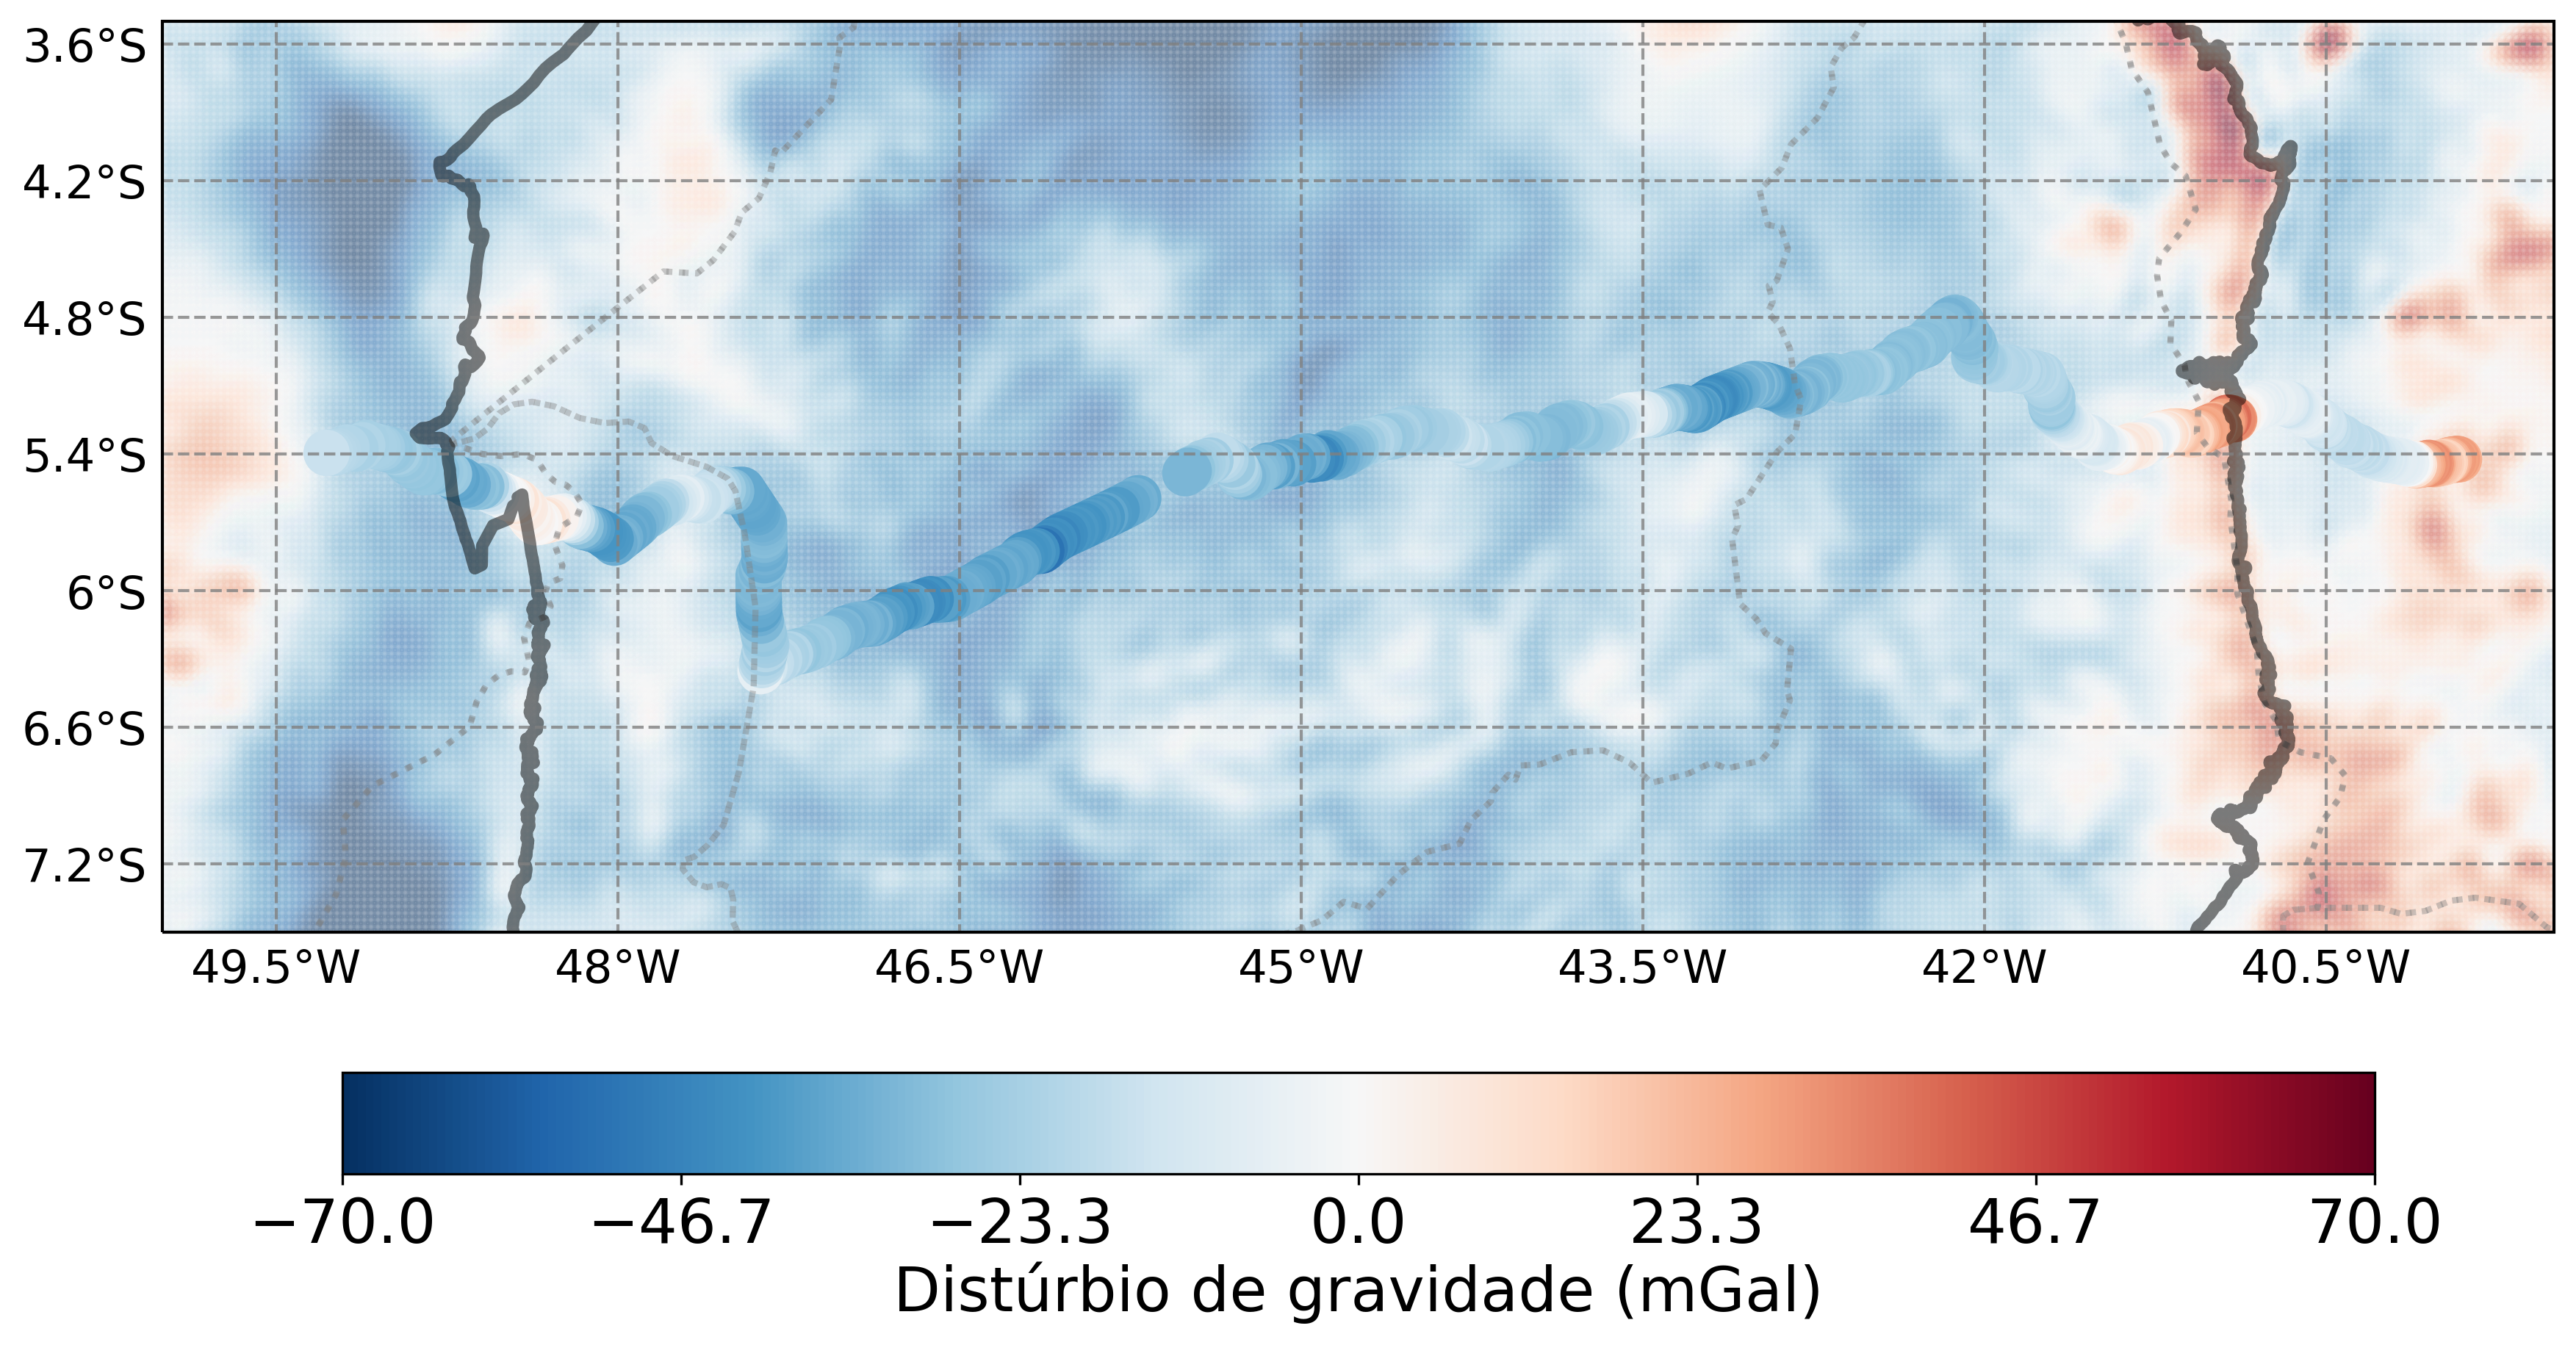
\includegraphics[scale=0.47]{figs/disturbio obs X pred.png}
	\caption{Imagem de $\delta g$ da região da Bacia do Parnaíba, sendo o contorno preto os limites desta, e o contorno pontilhado em cinza, o limite dos estados. Ao fundo, $\delta g$ predito pela malha regular gerada a partir dos valores de gravidade absoluta calculados pelo funcional \textit{gravity earth} e gravidade normal calculados pela fórmula analítica da gravidade, através da equação \ref{eq:disturbio}; sobrepondo, na forma do caminhamento terrestre, são $\delta g$ observados.}
	\label{fig:comparacao_delta}
\end{figure}


\begin{figure}[H]
	\centering
	\subfloat[Mapa com valores de $\delta g$ observados, com variação de $\pm57$ $mGal$ de acordo com a barra de cores, obtidos através da equação \ref{eq:disturbio}.]{\includegraphics[scale=0.37]{figs/perfil disturbio observado.png}}
	\
	\subfloat[Mapa com valores de $\delta g$ preditos, com variação de $\pm57$ $mGal$ de acordo com a barra de cores, obtidos através da equação \ref{eq:disturbio}.]{\includegraphics[scale=0.37]{figs/perfil disturbio predito.png}} 
	\
	\subfloat[Mapa de resíduo de $\delta g$ obtido pela diferença entre os distúrbios observados e preditos, apresentando uma variação de $\pm22.5$ $mGal$ de acordo com a escala de cores.]{\includegraphics[scale=0.37]{figs/perfil residuos.png}}
	\caption{Esquema comparativo de $\delta g$ observado, $\delta g$ predito e resíduos de $\delta g$. O contorno preto representa os limites da bacia do Parnaíba, e o contorno cinza, o limite dos estados.}
	\label{subfig:residuos_delta}
\end{figure}

Os resíduos de $\delta g$ apresentaram valores predominantemente positivos que se repetem com maior frequência entre as faixas branca e vermelha, segundo a escala de cores, que corresponde à variação $0$ a $\approx15$ mGal. Esta análise também leva à hipótese de que os dados preditos estão subestimados em relação aos observados. É provável que uma das causas também possa ser o truncamento dos harmônicos esféricos. No entanto, uma combinação de fatores também pode ser especulada. Lembrando que como o modelo \textit{EIGEN-6C4} é composto pela combinação de dados de diferentes origens, é relevante considerar que possa ter havido uma inclusão menos significativa de dados terrestres, uma vez que há uma baixa cobertura de dados no território brasileiro em comparação com outras localidades do planeta. Sendo assim, é possível pensar que o modelo \textit{EIGEN-6C4} seja menos acurado em determinadas regiões do globo, como na Bacia do Parnaíba. Para analisar estas subestimativas foi gerado o histograma da Figura \ref{subfig:histograma_delta}.a com média igual a $7.18$ $mGal$ e desvio padrão de $4.81$ $mGal$, onde se constata  resíduos predominantemente positivos. Essa análise corrobora a hipótese de dados calculados a partir do modelo estarem subestimados e evidenciam um erro de tendência. Foi gerado o gráfico de correlação da Figura \ref{subfig:histograma_delta}.b com valores de $\delta g$ observados e preditos para o levantamento, onde é possível constatar uma forte correlação  linear com $R^{2}$ igual à $0.92$, muito embora haja uma maior dispersão dos pontos em comparação com a análise feita para as altitudes geométricas (Figura \ref{subfig:histograma_h}.b). Além disso, nota-se que há uma densificação maior de pontos para valores negativos do que para positivos. 

\begin{figure}[H]
	\centering
	\subfloat[Histograma dos resíduos de $\delta g$, onde é possível observar um comportamento na média de $7.18$ $mGal$ e desvio padrão de $4.81$. A linha vermelha pontilhada corresponde ao hisograma de resíduos de $\delta g$ teórico, considerando uma distribuição gaussiana.]{\includegraphics[scale=0.245]{figs/histograma_residuos_delta.png}}
	\
	\,\,\subfloat[Gráfico de dispersão de $\delta g$, observado e predito, com ajuste linear representado pela reta vermelha com $R^{2}$ igual a $0.92$]{\includegraphics[scale=0.245]{figs/dispersao delta obs x pred.png}} 
	\caption{Esquema comparativo com histograma de resíduos de $\delta g$ ao lado do gráfico de correlação de $\delta g$ predito e $\delta g$ observados.}
	\label{subfig:histograma_delta}
\end{figure}

\section{Análise de dispersão complementar}

Foram gerados gráficos de correlação para complementar as análises anteriores a partir de $h$ e $\delta g$, e os resíduos de $h$ com resíduos de $\delta g$. A Figura \ref{subfig:h_delta}.a apresenta a correlação entre $\delta g$ observado e $h$ observada. Constata-se uma boa correlação linear entre as grandezas supracitadas, evidenciada pelo $R^{2} = 0.64$. Adicionalmente, observa-se uma maior dispersão para os menores valores de altitude e distúrbio de gravidade. Esse padrão não se repete para os maiores valores apresentados no gráfico, em decorrência da amostragem dos dados. É comum a associação de que regiões cujas altitudes são elevadas, possuem valores de gravidade menores. No entanto, o gráfico reflete o oposto, ou seja, em regiões de maiores altitudes, observamos distúrbios de gravidade igualmente elevados. E mais: são nestas regiões que a relação $h \times \delta g$ sofre menos dispersão. Pode-se inferir, portanto, que nessas regiões existe maior heterogeneidade de rochas em subsuperfície. As Figuras \ref{subfig:h_delta}.b e \ref{subfig:h_delta.b}.a apresentam a correlação entre $\delta g$ predito com $h$ predita e $\delta g$ predito com $h$ observado, respectivamente. Assim como a Figura \ref{subfig:h_delta}.a, existe certo padrão de correlação linear ($R^{2} = 0.64$). As amplitudes apresentam maior dispersão (i.e. menor correlação), mas, é possível constatar que os coeficientes de determinação apresentam pouca variação. Nas Figuras \ref{subfig:h_delta}.a, \ref{subfig:h_delta}.b e \ref{subfig:h_delta.b}.a é possível observar o padrão de maior adensamento de dados em altitudes menores, dada a baixa amostragem dos dados, referenciada anteriormente. A Figura \ref{subfig:h_delta.b}.b apresenta a correlação entre resíduos de $\delta g$ e de $h$. É notório que não existe qualquer correlação linear, dado o padrão bastante dispersivo associado ao baixo $R^{2}$ igual a $0.13$.

\begin{figure}[H]
	\centering
	\subfloat[Gráfico de dispersão de $\delta g$ observados com $h$ observado, apresentando um índice de determinação de $0.64$]{\includegraphics[scale=0.24]{figs/dispersao delta obs x h obs.png}}
	\
	\,\subfloat[Gráfico de dispersão de $\delta g$ preditos com $h$ predito, apresentando um índice de determinação de $0.67$]{\includegraphics[scale=0.24]{figs/dispersao delta pred x h pred.png}} 
	\caption{Esquema comparativo com gráficos de correlação entre $\delta g$ e $h$. A linha vermelha corresponde ao ajuste linear entre os parâmetros dos gráficos.}
	\label{subfig:h_delta}
\end{figure}
\begin{figure}[H]
	\centering
	\subfloat[Gráfico de dispersão de $\delta g$ predito com $h$ observado, apresentando um índice de determinação de $0.64$]{\includegraphics[scale=0.24]{figs/dispersao delta pred x h obs.png}}
	\	
	\subfloat[Gráfico de dispersão comparando os resíduos de $h$ com os resíduos de $\delta g$, apresentando um índice de determinação de $0.13$]{\includegraphics[scale=0.24]{figs/dispersao residuos.png}}
	\caption{Esquema comparativo com gráficos de correlação entre $\delta g$ predito e $h$ observado, e resíduos de $h$ com resíduos de $\delta g$. A linha vermelha corresponde ao ajuste linear entre os parâmetros dos gráficos.}
	\label{subfig:h_delta.b}
\end{figure}



% ------------------- capitulo 5:
\include{Conclusoes}

\bibliography{refs}

% ------------------- capitulo Apêncide:
%\include{Apendice}

\end{document}